
\chapter{Leveraging layout to process visually-rich documents}
\label{chapter:layout2pos}

\renewcommand{\leftmark}{\spacedlowsmallcaps{Leveraging layout to process visually-rich documents}}

\begin{chapabstract}
    {\em
    Due to their remarkable performance, general-purpose multimodal pre-trained language models have gained widespread adoption for Document Understanding tasks. The majority of pre-trained language models rely on serialized text, extracted using either Optical Character Recognition (OCR) or PDF parsing. However, accurately determining the reading order of visually-rich documents (VrDs) is challenging, potentially affecting the accuracy of the extracted text and leading to sub-optimal performance in downstream tasks. For information extraction tasks, where entity recognition is commonly framed as a sequence-labeling task, incorrect reading order can hinder entity labeling. In this work, we avoid reading order issues by discarding sequential position information. Based on the intuition that layout contains the information for correct reading order, we present Layout2Pos—a shallow Transformer designed to generate position embeddings from layout. Incorporated into a BART architecture, our approach demonstrates competitiveness with models dependent on reading order across three benchmark datasets for information extraction. We also show that evaluating models using a reading order different from the one seen during training can result in substantial performance drops, thereby highlighting the importance of not relying on the reading order of documents. \\
    \vspace*{5mm}

    The work in this chapter has led to the submission of a paper currently under review at NAACL 2024.}
    % \begin{itemize}
    %     \item \small \fullcite{}.
    % \end{itemize}
\end{chapabstract}

\ifthenelse{\boolean{skipCh7}}{\endinput}{}


\newpage

\minitoc
\chapterwithfigures{\nameref*{chapter:layout2pos}}
\chapterwithtables{\nameref*{chapter:layout2pos}}

% Textual content is organized in a specific layout to convey meaning and context. Layout holds considerable importance in conveying information, whether in business documents, scholarly papers, news articles or other written materials. 

The organization of textual content in a specific layout is crucial for conveying meaning and context, holding significant importance across various written materials, including business documents, scholarly papers, and news articles. In particular, layout determines the sequence in which text is intended to be read or processed within a document, \textit{i.e.}, the \textit{reading order}. A well-designed reading order ensures that readers can follow the logical flow and structure of information and comprehend the intended meaning of the text. However, defining a proper reading order is non-trivial due to the complexity of document layouts, which may include elements such as tables and multiple columns.

% \paragraph{Obtaining a Reading Order} 
When models are trained with a reading order that aligns with human understanding, they learn to capture the relationships between words, sentences, and paragraphs. Hence, reading order is crucial for models to perform well. Most pre-training methods for Document Understanding rely on serialized text, where either an \ac{OCR} engine or a PDF parser is used to extract text. However, due to the variety of layout formats, most \ac{OCR} engines and PDF parsers struggle to provide accurate reading orders, introducing \textit{serialization errors}. Serialization errors, \textit{i.e.}, noise that may arise during text extraction, such as misinterpretations or omissions, can lead to misalignments between the extracted text and the original visual content. For instance, an \ac{OCR} engine might misinterpret or introduce extraneous characters, while a PDF parser might misinterpret formatting elements or misorder words. 

Most of the time, the text extracted is re-arranged in a raster-scan order, aligning tokens from the top-left to the bottom-right corner \citep{clausner2013significance}. However, this linear organization does not always align with human reading patterns, particularly in documents with complex layouts such as multicolumn texts, tables, and forms. Serialization errors impact the accuracy of the extracted text and, therefore, affect the entire text processing pipeline. Without an accurate reading order, models may misinterpret the relationships between different parts of the text, resulting in suboptimal performance in downstream tasks. This poses a substantial challenge in various applications, notably in the field of Document Understanding, where document layouts can be complex. 

Furthermore, in real-word scenarios, documents may be processed by various \ac{OCR} engines for different reasons such as cost, availability, or integration with existing workflows. Each \ac{OCR} engine may have unique characteristics related to layout, font handling, or language support. These differences can introduce variations in the quality and accuracy of the \ac{OCR} output for the same document, impacting, most importantly, the reading order. This variability may result in significant fluctuations in downstream performance. However, it is crucial for organizations to be able to choose \ac{OCR} engines based on their specific requirements without compromising performance in downstream tasks.

% Furthermore, inaccuracies in \ac{OCR} outputs often require manual correction, which can be time-consuming and resource-intensive.

% \paragraph{Reading Order and Visual Information Extraction} 
In particular, in visual information extraction tasks, the primary goal\footnote{Additionally, the task extends to classifying the relationships between these recognized entities (\textit{relation extraction}). In this work, we do not focus on this task.} is to identify entities of predefined semantic types (\textit{e.g.}, names, dates, addresses). In this context, performance is notably impacted by serialization errors. Following the classic settings of \ac{NLP}, the task is commonly framed as a sequence-labeling problem. This approach involves labeling each token using a tagging scheme, such as BIO-tagging \citep{ramshaw1999text}, and leveraging these tags to identify entities, and leveraging these tags to identify entities. A sequence labeling-based approach operates under the assumption that each identified segment of an entity forms a continuous sequence of words within the input. While this assumption is valid for plain texts, it may not hold for real-world documents, where \ac{OCR} systems or PDF parsers might not correctly organize text. For instance, an entity might be split into non-continuous fragments. Such disordered input disrupts the BIO-tagging scheme, preventing the models from accurately identifying entities. Moreover, for training sequence labeling approaches, word-level annotations are essential. However, they are not always available; some datasets only provide the text corresponding to each information type \citep{gralinski2020kleister}. Obtaining word-level annotations involves matching these texts with the words in the document, which can be time-consuming if done manually or susceptible to errors if performed automatically.

% Current state-of-the-art approaches require labeling of every word, which is costly to obtain, and consequently not available for many real life tasks. The distinction between endto-end data and data labeled on the word level is subtle but important. In the invoice example the end-to-end data simply tells us what the total is, whereas data labeled on the word level tells us where it is. The former type of data is plentiful, produced naturally and is hard to learn from. The latter is scarce, must be explicitly produced for the purpose of machine learning, and is easier to learn from.

% \paragraph{On the Role of Layout in Determining Reading Order} 
On the other hand, layout inherently encapsulates the correct reading order of documents by visually organizing content in a structured manner. A well-designed layout guides the reader's natural progression from one section to another, ensuring coherent and logical information flow. Therefore, understanding the layout provides essential cues for determining the correct reading order, as it aligns with the visual hierarchy and structure intended by document creators. 

Yet, existing pre-training methods for Document Understanding often neglect this aspect, opting to oversimply the integration of layout. For instance, LayoutLM \citep{xu2020layoutlm} incorporates layout information as an extra embedding in the input layer, while LayoutLMv2 \citep{xu2020layoutlmv2} adds it as a bias term in the attention layer. Although ERNIE-Layout \citep{peng2022ernie} learns the relationship between layout and reading order through a pre-training strategy involving reading order prediction, it continues to rely on sequential position embeddings derived from the reading order obtained via \ac{OCR}. However, by investigating the position-awareness in causal language models with no explicit positional encodings, \citet{haviv2022transformer} show that these models develop an implicit understanding of absolute positions to compensate for missing information. It is suggested that causal attention, a mechanism in which each token attends only to its preceding positions in a sequence, allows the model to estimate the number of predecessors each token can attend to, thereby approximating its absolute position. Our objective is to demonstrate that the capability of a model to approximate its absolute position is not restricted to causal models, but holds true across various scenarios when layout information is provided.

% \paragraph{Generative Approaches for Visual Information Extraction} 
Unlike sequence labeling approaches that entirely depend on the content extracted via \ac{OCR}, generative models can bypass the need for word-level annotations and generate text without being restricted by the document's content or its reading order, enabling them to potentially correct \ac{OCR}-induced errors. \citet{sage2020end} represent the information to be extracted as a sequence of tokens in the XML language. They employ a recurrent encoder-decoder architecture to generate XML representations, using pointer-generator networks \citep{see2017get} to allow the model to dynamically decide whether to generate a word from its vocabulary or copy it directly from the document. \citet{townsend2021doc2dict} use a Transformer \citep{vaswani2017attention} language model trained on database records to generate JSON-like representation of the extracted information. In close relation to our work, TILT \citet{powalski2021going} is a Transformer encoder-decoder model enhanced with layout and visual information, specifically designed for visual information extraction tasks. Instead of relying on \ac{OCR} for text extraction, Donut \citep{kim2022ocr} uses a Transformer visual encoder to extract features from a document image. A textual Transformer decoder is then used to map these features to a desired structured format, such as JSON, for visual information extraction tasks. In contrast to Donut, our method does not rely on visual features, providing better computational efficiency when various information extraction tasks are conducted or/and complex documents are processed. \\

% In particular, Visual Information Extraction heavily relies on the detected text and reading order provided by \ac{OCR}. Inaccuracies in the reading order can disrupt the structure of the extracted data, leading to issues such as entities being split into non-contiguous fragments. Besides, the task is commonly framed as a sequence labeling task, and common labeling schemes used to annotate entities in a sequence for sequence labeling, such as the BIO-tagging scheme \citep{ramshaw1999text}, entirely depend on the detected reading order. Furthermore, in the context of sequence labeling, the model's output is restricted to the detected words. As a consequence, there might be no exact match for the expected value in a document. 

In this chapter, we focus on mitigating serialization errors by \textit{entirely discarding sequential position information}. We introduce \textit{Layout2Pos}, a shallow Transformer model designed to generate position embeddings from the document layout. Our endeavor is twofold: from a practical standpoint, we aim to enhance the robustness of models to reading order changes, crucial for real-world applications; from a theoretical perspective, we demonstrate that it is feasible to discard sequential position information without compromising overall performance. We integrate this module into a sequence-to-sequence framework. To train the model, the language modeling task is coupled with a pre-training strategy designed to instill the model with the ability to learn the reading order from layout information. This integration eliminates the reliance on reading order and enables the generation of values that are not explicitly present in the input. We demonstrate the benefits of our approach for visual information extraction tasks, showcasing competitive performance to models that depend on reading order.


\section{Reconstructing Positional Information from 2D Positions}

In this section, we present preliminary experiments that underscore the limitations inherent to \ac{OCR} procesing in terms of accurately preserving the reading order of tokens. In response to the challenges posed by \ac{OCR}-induced serialization errors, we then introduce a novel approach named Layout2Pos. This module goes beyond conventional approaches by discarding the reliance on reading order information. Instead, Layout2Pos leverages the inherent 2D positional information of tokens within the document page to reconstruct sequential positional information, thereby enhancing the robustness and reliability of downstream tasks.

\subsection{Preliminary Experiments: OCR Serialization Errors}

To gauge the extent of \ac{OCR}-induced serialization errors, we conduct preliminary experiments comparing the annotated ground-truth reading order against the reading orders produced by 1) Tesseract OCR \citep{kay2007tesseract}, a widely-used \ac{OCR} engine, and 2) DocTR \citep{doctr2021}, an \ac{OCR} engine based on deep learning models. The goal is to assess the alignment of the reading order produced via \ac{OCR} with the actual human reading patterns.

We use a subset of 100 documents from the ReadingBank \citep{wang2021layoutreader} dataset. ReadingBank is a benchmark dataset for reading order detection that includes high-quality reading order annotations extracted from Word documents. These annotations capture the correct sequence of words as visually presented in the documents. Upon examination of the samples and discerning patterns that appear most frequently, we have identified four prevalent document layout types: \textit{plain} layout, \textit{lists}, \textit{multicolumn} layout, and \textit{tables}. We provide examples in Figure~\ref{fig:layout-examples}. 

Tesseract OCR and DocTR are employed to extract and serialize text from the documents. The reading orders produced are compared against the ground-truth for discrepancies. Specifically, we evaluate accuracy by comparing, for each word in the ground-truth sequence, the actual next word with the one predicted by each \ac{OCR} engine. We compute the accuracy obtained by each system for each specific layout type. Results are reported in Table~\ref{table:ocr-preliminary-experiments}. Additionally, we include the results obtained by our approach, Layout2Pos. Our findings indicate that both \ac{OCR} engines face increased difficulty in reconstructing the correct reading order as the document layout becomes more complex.\footnote{This difficulty in accurately predicting the next word is further attributed to the \ac{OCR} engines' misinterpretation of certain words.} Our approach exhibits a similar trend, although to a significantly lesser degree. Furthermore, it demonstrates higher accuracy for each document type compared to both OCR engines.

Additionally, we provide the ground-truth reading order and the reading order generated by Tesseract OCR for a sample table (Figure~\ref{fig:reading-orders-table}) and a document with a multi-column layout (Figure~\ref{fig:reading-orders-multicolumn}). In the case of the table, a comparison with the ground-truth reading order reveals that Tesseract OCR lacks knowledge about cells, as it organizes text in a top-left to bottom-right manner. Regarding the document with two columns, Tesseract OCR reads the text column by column, despite the document being horizontally divided into subgroups. This observation highlights the limited understanding of structure by \ac{OCR} engines. 

These preliminary experiments provide the groundwork for investigating into novel approaches designed to alleviate serialization errors, ultimately enhancing the performance of document understanding models.

\begin{figure}
    \centering
    \small
      \begin{subfigure}[b]{0.24\textwidth}
        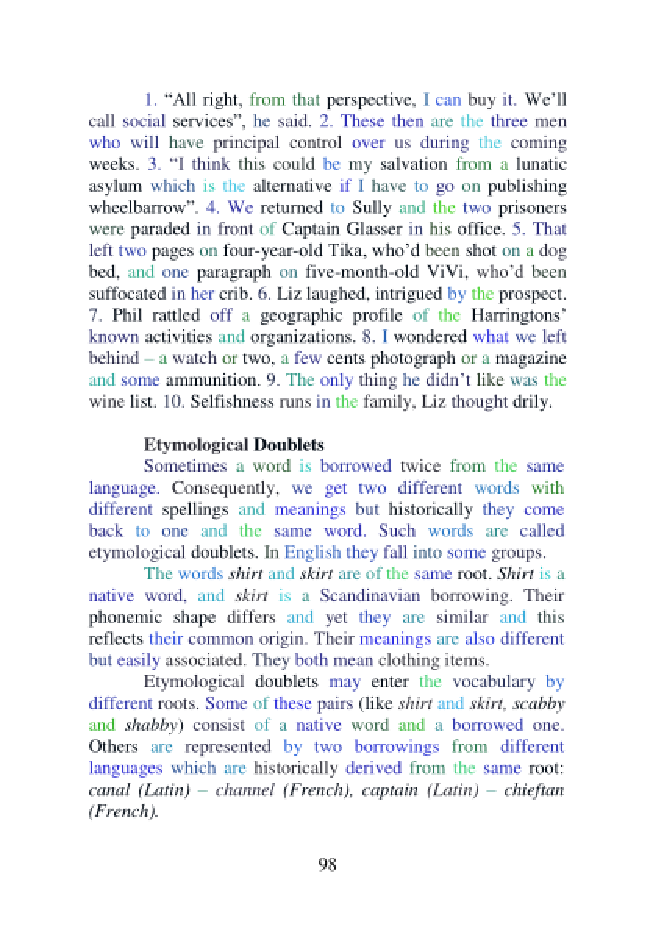
\includegraphics[width=\textwidth]{images/chapter4/plain.pdf}
        \caption{Plain}
      \end{subfigure}
      \begin{subfigure}[b]{0.24\textwidth}
        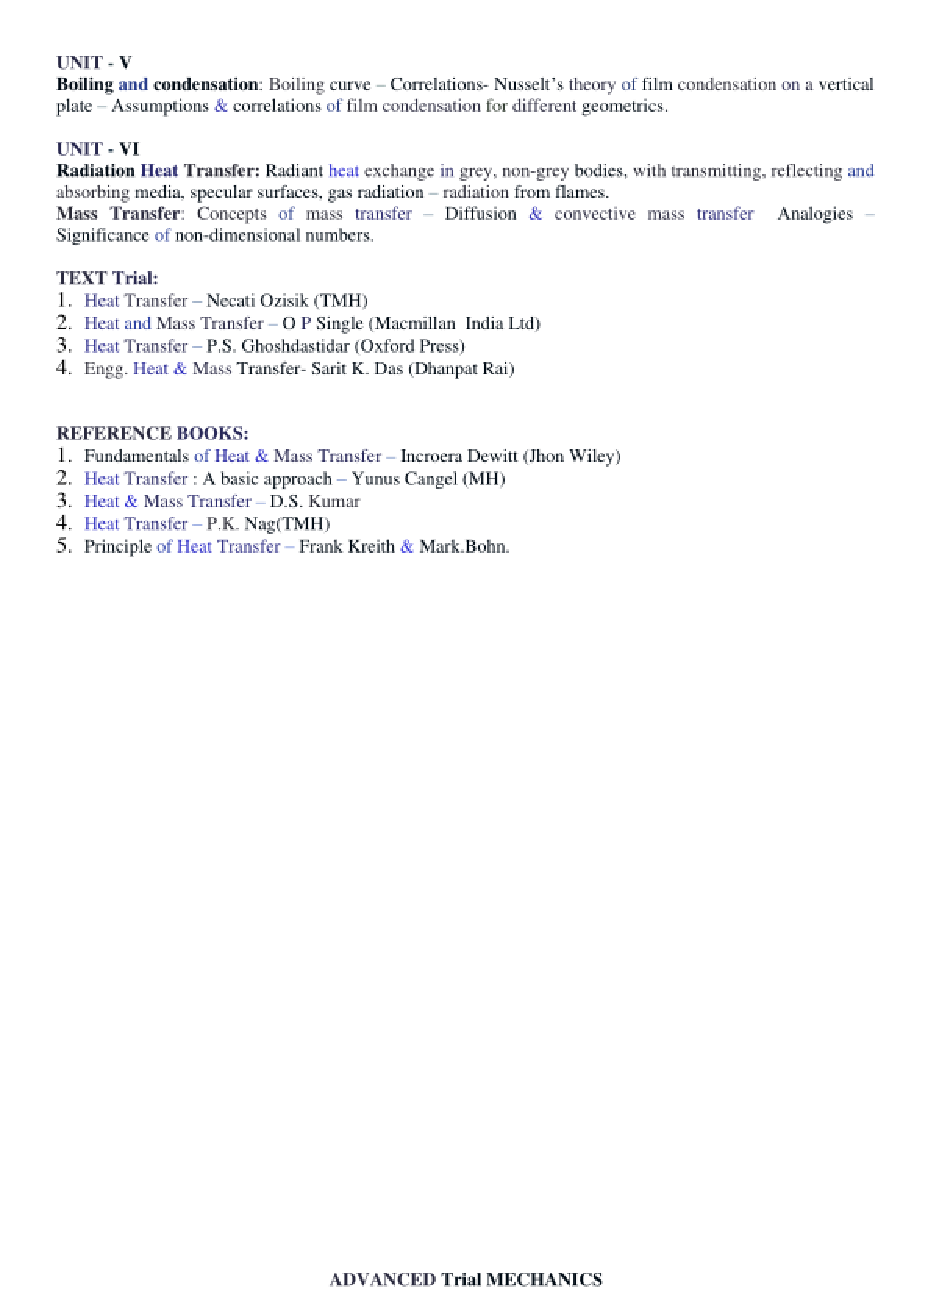
\includegraphics[width=\textwidth]{images/chapter4/list.pdf}
        \caption{List}
      \end{subfigure}
      \begin{subfigure}[b]{0.24\textwidth}
        
\includegraphics[width=\textwidth]{images/chapter4/multicolumn.pdf}
        \caption{Multicolumn}
      \end{subfigure}
      \begin{subfigure}[b]{0.24\textwidth}
        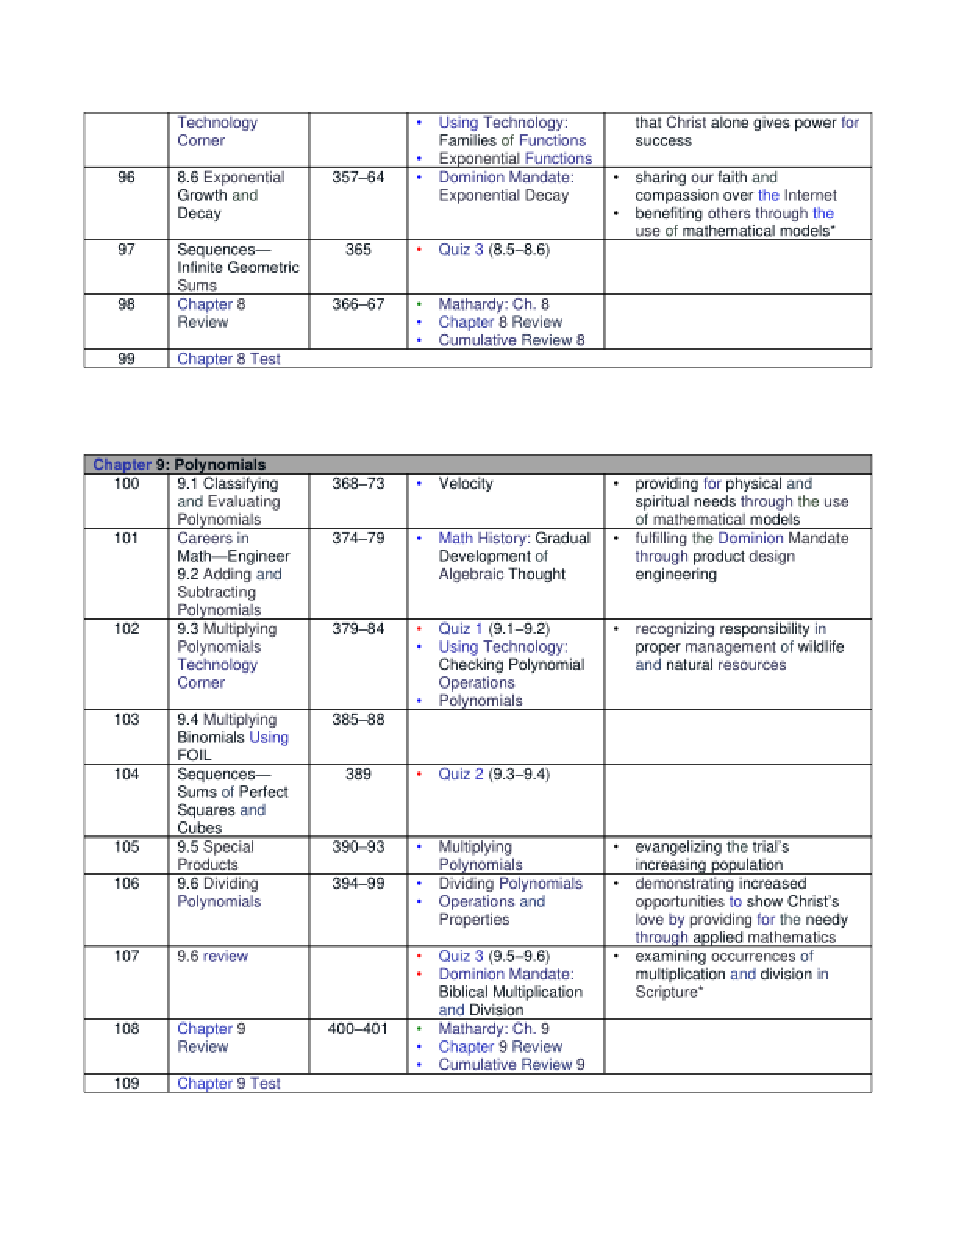
\includegraphics[width=\textwidth]{images/chapter4/tables.pdf}
        \caption{Table}
      \end{subfigure}
    \caption{Examples of documents for each layout category, arranged from the simplest to the most complex.}
    \label{fig:layout-examples}
\end{figure}

\begin{table}
  \centering
  \small
  \begin{adjustbox}{max width=\textwidth}
  \begin{threeparttable}
  \begin{tabular}{lcccccccc}
      \toprule
          & & \multicolumn{4}{c}{\textbf{Layout Type}} & \\
          & & \textbf{Plain} & \textbf{Lists} & \textbf{Multicolumn} & \textbf{Tables}\\
      \midrule
      Tesseract OCR \citep{kay2007tesseract} & & 78.71 & 72.75 & 61.43 & 36.97 \\
      DocTR \citep{doctr2021} & & 86.83 & 77.83 & 82.54 & 66.11 \\
  \bottomrule
  \end{tabular}
  \end{threeparttable}
  \end{adjustbox}
  \caption{Accuracy (in \%) obtained by each \ac{OCR} engine, for each document layout type.}
  \label{table:ocr-preliminary-experiments}
\end{table}

\begin{figure}
    \centering
    \small
      \begin{subfigure}[b]{\textwidth}
        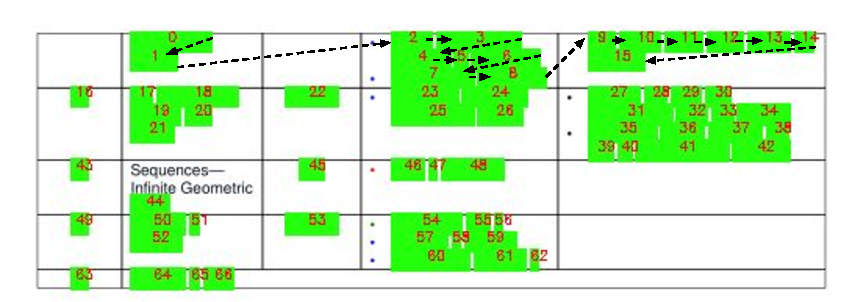
\includegraphics[width=\textwidth]{images/chapter4/gold_tables_with_ro.pdf}
        \caption{Ground-truth reading order}
      \end{subfigure}
      \begin{subfigure}[b]{\textwidth}
        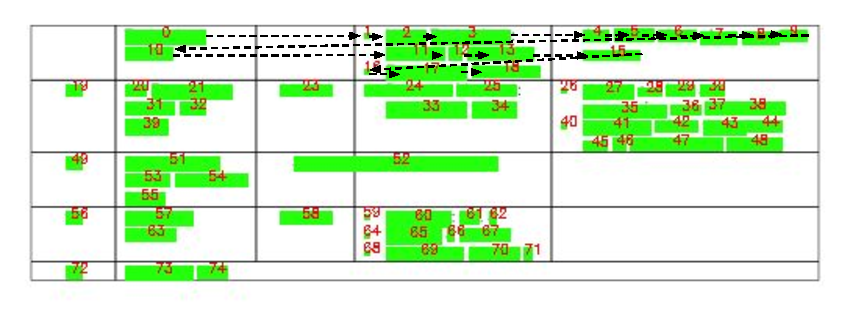
\includegraphics[width=\textwidth]{images/chapter4/tesseract_tables_with_ro.pdf}
        \caption{Reading order obtained through Tesseract}
      \end{subfigure}
    \caption{Ground-truth reading order (a) compared to the reading order generated by Tesseract (b) for a sample table. Arrows emphasize the difference in reading order in the first row. Non-highlighted text indicates that it does not appear in the serialized sequence.}
    \label{fig:reading-orders-table}
\end{figure}

\begin{figure}
  \centering
  \small
      \begin{subfigure}[b]{0.4\textwidth}
        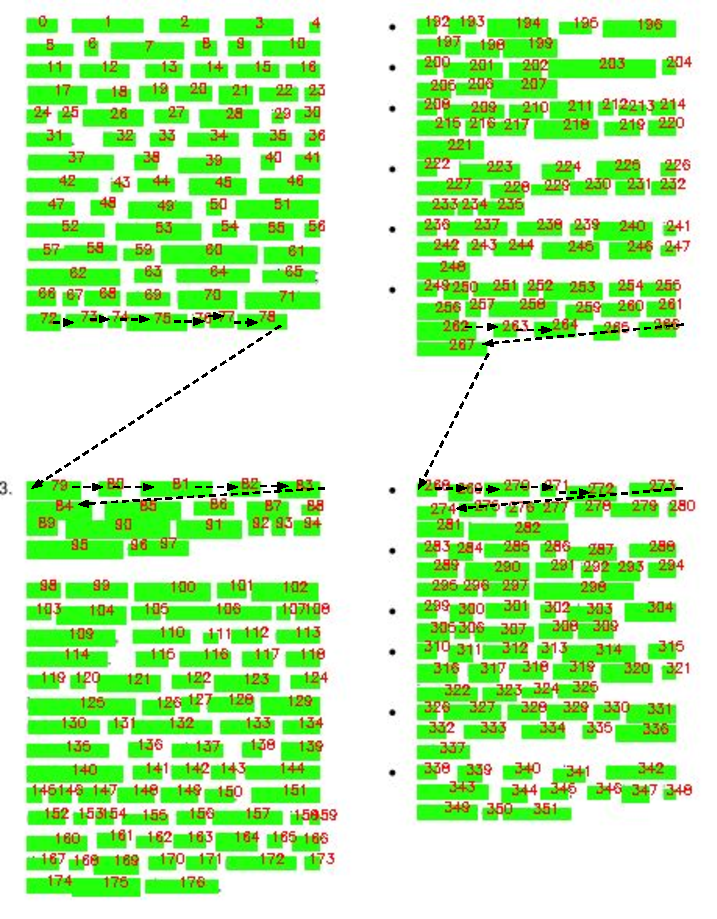
\includegraphics[width=\textwidth]{images/chapter4/gold_multicolumn_with_ro.pdf}
        \caption{Ground-truth}
      \end{subfigure}
      \begin{subfigure}[b]{0.4\textwidth}
        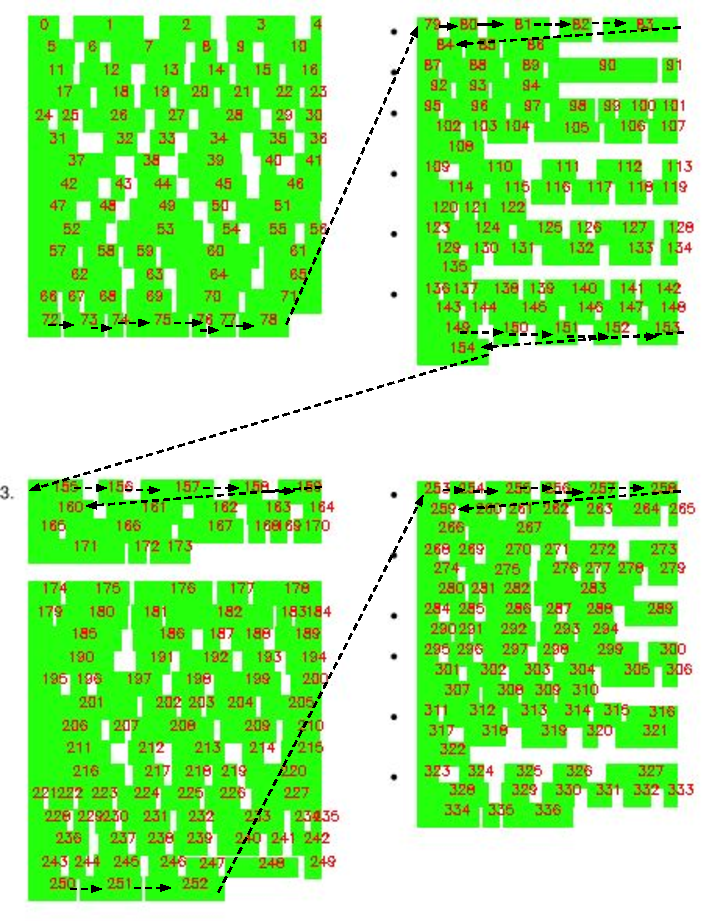
\includegraphics[width=\textwidth]{images/chapter4/tesseract_multicolumn_with_ro.pdf}
        \caption{Tesseract}
      \end{subfigure}
    \caption{Ground-truth reading order (a) compared to the reading order generated by Tesseract (b) for a document with a two-column layout. The document was cropped for better visibility. Arrows emphasize the difference in reading order. Non-highlighted text indicates that it does not appear in the serialized sequence.}
    \label{fig:reading-orders-multicolumn}
\end{figure}


\subsection{Layout2Pos Module}

Building on the insights gained from the previous experiment, accurately retrieving the correct reading order poses a significant challenge for \ac{OCR} engines. We argue that it is possible to retrieve the correct reading order by leveraging document layout. To address this, we propose a novel approach, \textit{Layout2Pos}, a transformer-based module that does not rely on the reading order generated by OCR, and learns position embeddings solely from the spatial positions of tokens. In the following, we elaborate on the process of encoding spatial information into layout embeddings, followed by an in-depth description of our Layout2Pos module.

% Layout2Pos is a stack of Transformer layers designed to generate a corresponding sequence of 1D position embeddings based on spatial information. 

\subsubsection{Encoding Layout Information}

To encode layout information, we use 1) bounding box information, 2) 2D relative positions, and 3) a novel method based on line and column relative positions.

\paragraph{Encoding Bounding Box Information} 

The spatial position of a token is represented by its bounding box in the document page image, denoted as $(x_0, y_0, x_1, y_1)$, where $(x_0, y_0)$ and $(x_1, y_1)$ correspond to the coordinates of the top-left and bottom-right corners, respectively. Following LayoutLMv2, we discretize and normalize these coordinates to integers within the range of $[0, ..., 1000]$. Four embedding tables are employed to encode spatial positions: $\text{LE}_x$ and $\text{LE}_y$ for the coordinate axes ($x$ and $y$), and $\text{LE}_w$ and $\text{LE}_h$ for the bounding box size (width and height). In line with LayoutLMv2, the final layout embedding $\bell \in \mathbb{R}^{d}$ of a token, whose bounding box is $(x_0, y_0, x_1, y_1)$, is defined as follows~($\mathbin\Vert$ denotes concatenation):

\begin{equation}
  \begin{split}
      \bell & = \text{LE}_x(x_0) \mathbin\Vert \text{LE}_y(y_0) \\
      & \mathbin\Vert \text{LE}_x(x_1) \mathbin\Vert \text{LE}_y(y_1) \\
      & \mathbin\Vert \text{LE}_w(x_1 - x_0) \\
      & \mathbin\Vert \text{LE}_h(y_1 - y_0), 
  \end{split}
\label{eq:layout-embeddings}
\end{equation}

\paragraph{Leveraging 2D Relative Positions} 

LayoutLMv2 encodes spatial relative positions as bias terms added to the attention scores to explicitly capture the spatial relationship between tokens (see Section~\ref{section:related-document-understanding-layout-aware-attention}). Following LayoutLMv2, for each pair of bounding boxes $((x_0, y_0, x_1, y_1), (x^{\prime}_0, y^{\prime}_0, x^{\prime}_1, y^{\prime}_1))$, we compute the horizontal distance $x^{\prime}_0 - x_0$ between the left edge of each box and the vertical distance $y^{\prime}_1 - y_1$ between the bottom edge of each box. 

In addition, we provide additional insights into the spatial relationships of tokens by computing the horizontal distance $x^{\prime}_1 - x_0$ between the right edge of one box and the left edge of the other (indicating information about the combined length). Furthermore, we calculate the horizontal distance $x^{\prime}_1 - x_1$ between the right edge of each box, providing information about the length of the second token in the pair. 

\paragraph{Incorporating Line and Column Relative Positions}

Understanding the relative positions within columns provides information about the sequential structure of the document, aiding in distinguishing between different parts of the document. On the other hand, the relative positions within lines is valuable for documents with multicolumn layouts, offering insights into the spatial arrangement of text across columns. Hence, for each bounding box, we identify other bounding boxes that share the same line/column. This is determined by whether the horizontal/vertical line passing through the center of the box intersects with the other bounding boxes. If there is an intersection, the boxes are considered to be on the same line/column. For each token $t_i$, we determine its positions $p^{(l)}(i)$ and $p^{(c)}(i)$ within its corresponding line and column, using a left-to-right order for lines and a top-to-bottom order for columns. Then, we compute the relative sequential distance $\delta^{l}_{ij}$ and $\delta^{c}_{ij}$ between elements within each line and column. If they do not belong to the same line or column, the distance is set to $\infty$. 

Let us summarize formally how attention is computed. Suppose $\bm{q}^{\ell}_i$ and $\bm{k}^{\ell}_i$ denote the query and key projections obtained from the layout embedding $\bell_i$ of token $i$. Let $\bm{b}^{(2D_x)}$, $\bm{b}^{(2D_y)}$, $\bm{b}^{(l)}$, and $\bm{b}^{(c)}$ be the horizontal, vertical, line, and column relative position biases, respectively. In Layout2Pos, attention is re-defined as:

\begin{equation}
  \begin{split}
  \alpha_{ij} &= \dfrac{1}{\sqrt{d}} \left(\bm{q}^{\ell}_i \cdot \bm{k}^{\ell}_j\right)
              + \bm{b}^{(2D_x)}_{x^{(j)}_{0} - x^{(i)}_{0}} + \bm{b}^{(2D_y)}_{y^{(j)}_{1} - y^{(i)}_{1}} \\
              & + \bm{b}^{(2D_x)}_{x^{(j)}_{1} - x^{(i)}_{0}} + \bm{b}^{(2D_x)}_{x^{(j)}_{1} - x^{(i)}_{1}} 
               + \bm{b}^{(l)}_{\delta^{l}_{ij}}  + \bm{b}^{(c)}_{\delta^{c}_{ij}}
  \end{split}
\label{eq:layout2pos-attention}
\end{equation}

% \noindent The relative sequential distances between elements within lines and columns, $\bm{\delta}^{(line)}$ and $\bm{\delta}^{(column)}$, are defined as follows:

% \begin{equation}
%   \begin{split}
%     \delta^{l}_{ij} &= 
%         \begin{cases}
%           posInLine(j) - posInLine(i), & \text{if } line(j) = line(i)\\
%           \infty,              & \text{otherwise}.
%         \end{cases} \\
%     \delta^{c}_{ij} &= 
%       \begin{cases}
%         posInColumn(j) - posInColumn(i), & \text{if } column(j) = column(i)\\
%         \infty,              & \text{otherwise}.
%       \end{cases}
%   \end{split}
% \end{equation}

\subsubsection{Learning Position Embeddings from Layout Information}

\begin{figure}
  \centering
  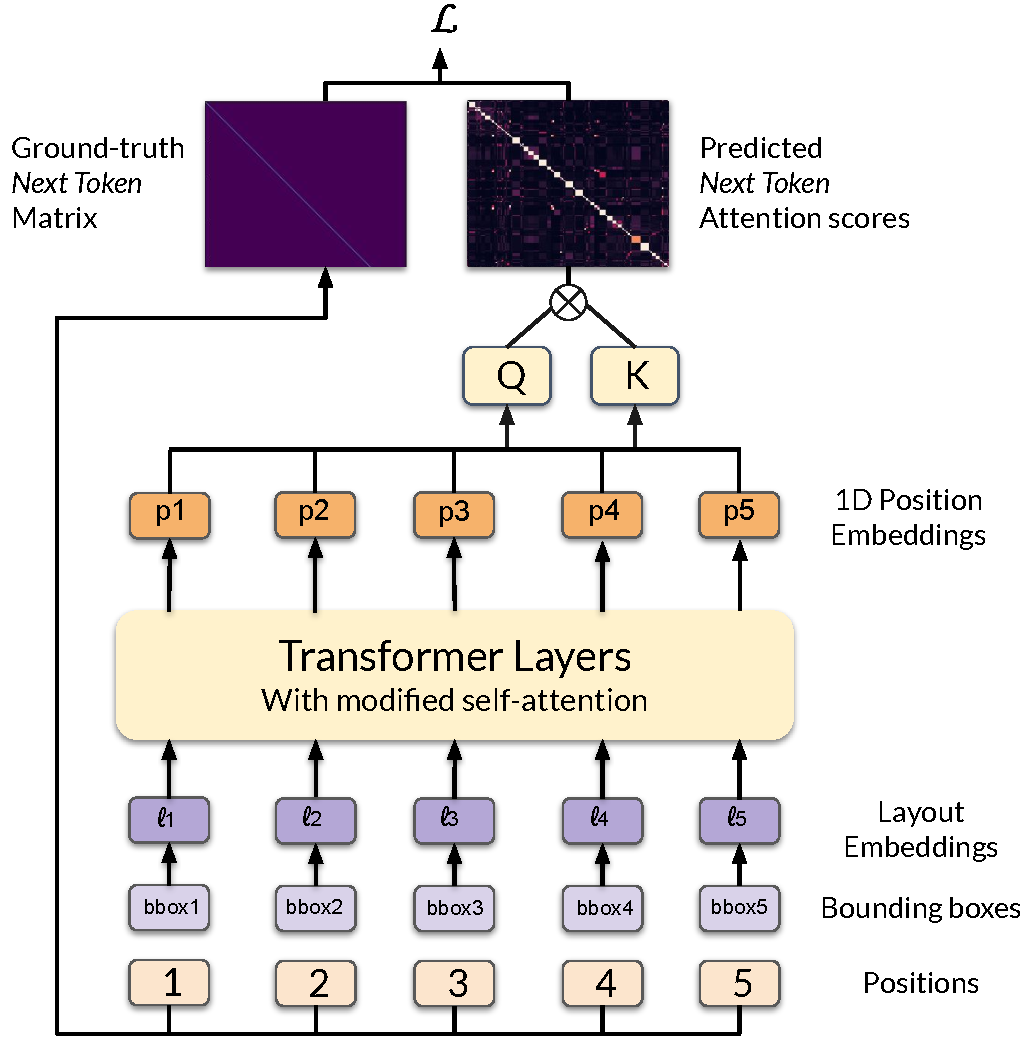
\includegraphics[width=0.6\textwidth]{images/chapter4/Layout2Pos.pdf}
  \caption{Layout2Pos Architecture.}
  % \caption{Layout2Pos Architecture. The input consists of a sequence of token bounding box coordinates, transformed into corresponding embedding sequences. Self-attention in the stack of Transformer layers is modified as defined by Equation~\ref{eq:layout2pos-attention}. $\bm{Q}$ and $\bm{K}$ are the queries and keys obtained by projecting the position embeddings. The attention scores obtained through dot-product are compared against the ground-truth matrix to compute the Next Token Position Prediction loss.}
  \label{fig:layout2pos-module}
\end{figure}

Given a sequence of layout embeddings derived from token bounding box coordinates, as defined by Equation~\ref{eq:layout-embeddings}, Layout2Pos employs a stack of Transformer layers to contextualize the sequence. The outputs of the last layer, $\bm{\overline{\bell}_i}$, serve as position embeddings, \textit{i.e.}, $\bm{p}_i = \bm{\overline{\bell}_i}$. The objective is for these embeddings $(\bm{p}_1, \cdots, \bm{p}_n)$ to carry information regarding the reading order. To accomplish this, we build a simple classifier on top of these embeddings, designed to compute alignment scores between each token:

\begin{equation}
  A_{ij} = \left(\bm{p}_i \bm{W}^q\right)\left(\bm{p}_j \bm{W}^k\right).
\end{equation}

\noindent We assume that the attention matrix $\bm{A}$ carries information about the reading order, \textit{i.e.}, $A_{ij}$ represents the probability that the $j$-th token follows the $i$-th token. Let $N$ denote the ground-truth binary matrix obtained from the ground-truth reading order, where $N_{ij}$ equals $1$ if token at position $j$ is the \textit{next} token after token at position $i$ in the sequence, and $0$ otherwise. We define the \textit{Next Token Position Prediction} strategy, which consists in using the attention matrix $\bm{A}$ to predict the next token of each token in the sequence (\textit{next token matrix}). The corresponding cross-entropy loss is defined as follows:

\begin{equation}
  \mathcal{L}_{NTPP} = - \dfrac{1}{n} \sum_{i=1}^n \sum_{j=1}^n \bm{N}_{ij} \log\left(\textrm{softmax}_i(\bm{A}_{\cdot j})\right)
\end{equation}

\noindent As such, Layout2Pos can be trained to capture the relationship between layout and reading order \footnote{It is noteworthy that a global reading order is unnecessary; there is no requirement to establish an order between two words that belong to segments that have no relation to each other.} by ensuring that the attention matrix $\bm{A}$ derived from the computed position embeddings $(\bm{p}_1, \cdots, \bm{p}_n)$ carries information about the next token for each token in the sequence. The architecture of Layout2Pos is depicted in Figure~\ref{fig:layout2pos-module}. 

% Given that each token is treated as a bounding box defined by its size and position, a significantly smaller representation space can be chosen for layout features compared to text. As Layout2Pos does not need to understand semantic content, it may require a smaller latent space dimension than conventional multimodal pre-trained models. 

\subsubsection{Integrating Layout2Pos into a Sequence-to-Sequence Framework}

\begin{figure}
  \centering
  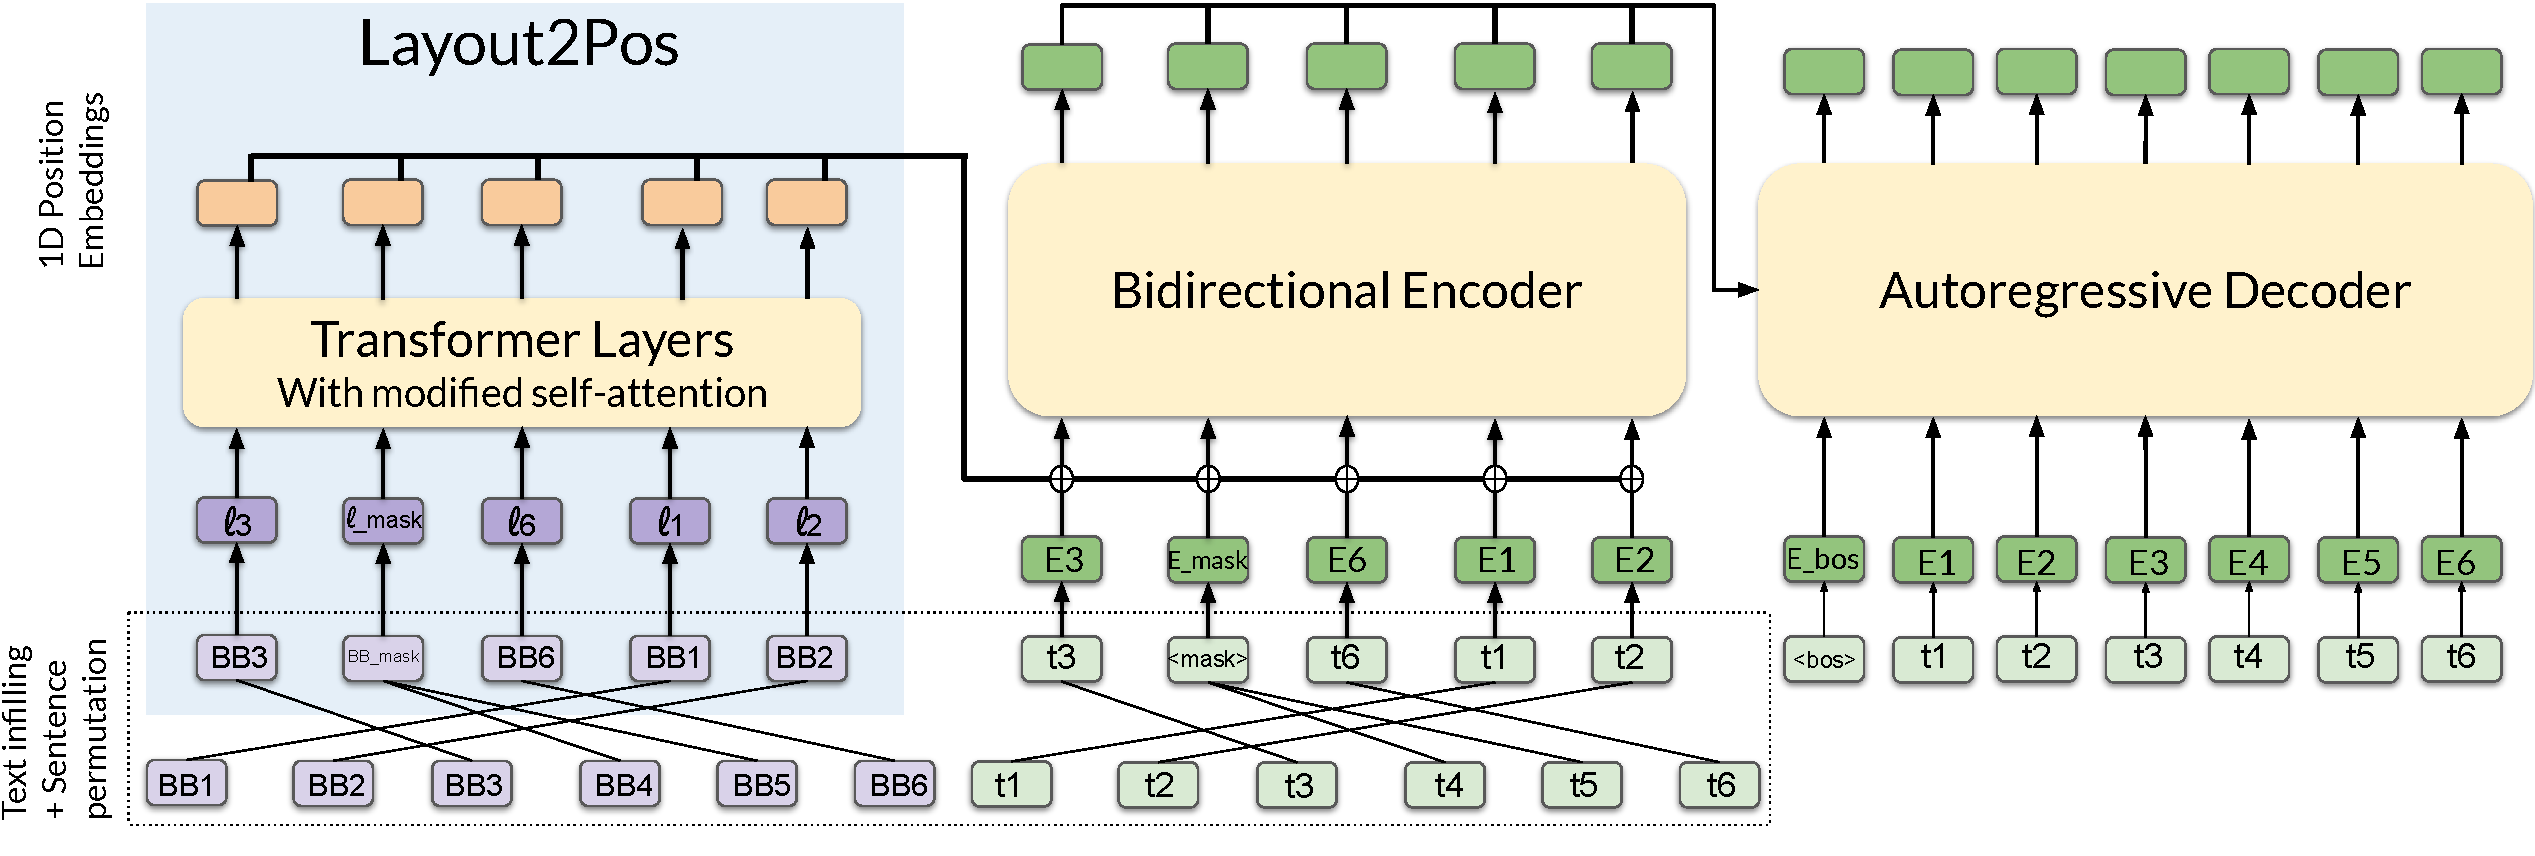
\includegraphics[width=\textwidth]{images/chapter4/Layout2Pos+BART.pdf}
  \caption{Architecture of Layout2Pos integrated into a BART model, \textit{i.e.}, BART+Layout2Pos. The input consists of two components: a sequence of tokens and a sequence of token bounding box coordinates.}
  \label{fig:layout2pos-ed}
\end{figure}

Layout2Pos can be integrated into any language model, removing the reliance on sequential position information. This is achieved by substituting the traditional position encodings derived from \ac{OCR} by Layout2Pos' position embeddings. Specifically, we integrate Layout2Pos into a Transformer encoder-decoder architecture, as illustrated in Figure~\ref{fig:layout2pos-ed}. The model takes as input a sequence of tokens and their associated bounding boxes, both embedded using embedding tables (Section~\ref{section:related-pretrained-language-models-bert}). The sequence of position embeddings, obtained by Layout2Pos, is added to the sequence of token embeddings. The resulting sequence is input to the bidirectional encoder. The output sequence of contextualized embeddings is fed to the autoregressive decoder to generate the target sequence.


\paragraph{Corruption Loss} Layout2Pos is trained together with the encoder-decoder model. While the module learns to predict the subsequent token of each token based on layout information, the encoder-decoder follows a pre-training approach similar to \ac{BART} \citep{lewis2019bart}. The model is trained to reconstruct the original input sequence from a corrupted version (\textit{denoising}). Sequences are corrupted by randomly replacing text spans with a single mask token (\textit{text infilling}) and permuting sentences (\textit{sequence permutation}). The corrupted sequence is encoded using the bidirectional encoder, and the autoregressive decoder is trained to reconstruct the original sequence. The final loss is expressed as follows:

\begin{equation}
  \mathcal{L} = \mathcal{L}_{NTPP} + \mathcal{L}_{Denoising}.
\end{equation}

\noindent We refer to the overall model as BART+Layout2Pos. 


\paragraph{Inference for Information Extraction Tasks} To determine how the model predicts the next token of the sequence for information extraction tasks, we employ a customized variant of beam search to generate tokens while minimizing repetitions, therefore enhancing the coherence of the generated sequences. In this modified version, the generated tokens, if present in the source sequence, are constrained not to occur more frequently than in the original source. This constraint is enforced by keeping count of the number of occurrences of each token in the source sequence within the target sequence, masking the corresponding logit when the maximum occurrence is reached and redistributing the probability mass over the valid tokens. 


\section{Experiments}

In this section, we provide an overview of the datasets used for pre-training our models and conducting visual information extraction tasks. Furthermore, we provide details on the experimental setup, covering baselines, pre-training methodologies, and fine-tuning protocols. 

% To valid our position embeddings, we evaluate our model on the Next Token Position Prediction task. Finally, we analyze how it behaves on three benchmark visual information extraction tasks. 

\subsection{Data}

\subsubsection{Pre-training Data}

Following a common practice in the field of Document Understanding, we collect data from the IIT-CDIP collection \citep{lewis2006building} to build our pre-training dataset (Section~\ref{section:related-document-understanding-pretraining}). IIT-CDIP consists of around 11 million document page images of various types and layouts, including news articles, scientific reports, handwritten materials, and more. The collection contains scanned images of documents, introducing challenges related to image quality, resolution, and potential artifacts. As such, we leverage IIT-CDIP to pre-train models under realistic conditions. We select over 7 million document images from the collection to build our pre-training dataset, allocating over 18k for validation, another 18k for testing, and the remaining images for training. To extract text and bounding boxes from the documents, we use DocTR \citep{doctr2021}. Due to potential serialization errors induced by DocTR, and given that the Next Token Position Prediction task requires documents with proper reading orders, IIT-CDIP is only used for training models in language modeling tasks (\textit{i.e.}, denoising). 

To enable Layout2Pos to effectively learn the correct reading order of documents, we use the 500k documents from ReadingBank \citep{wang2021layoutreader}. These documents are serialized and annotated with high-quality reading order annotations, serving as the training data for both Next Token Position Prediction and language modeling tasks. 

Our final pre-training corpus is referred to as IIT-CDIP+ReadingBank. While permutation is used for both datasets, text infilling is not applied to ReadingBank. This choice is made to prevent potential alignment issues between Next Token Position Prediction and language modeling, which could arise from replacing spans of tokens with a single mask token.

In cases where a word is split into multiple tokens, earlier approaches based on word-level bounding boxes typically assign the word's bounding box to all the tokens within that word. However, this approach is inefficient for Next Token Position Prediction, given that tokens within the same word would share identical layout embeddings, hence hindering accurate predictions of the next token. Therefore, we approximate token-level bounding boxes by dividing each word-level bounding box by the number of characters in the word. 

\subsubsection{Data for Visual Information Extraction}

We evaluate our approach on visual information extraction tasks, where the goal is to extract semantic entities from visually-rich documents, based on a set of pre-defined keys. This evaluation is conducted using three benchmark for visual information extraction (Section~\ref{section:related-document-understanding-visual-information-extraction}), each covering different document types: FUNSD \citep{jaume2019funsd}, SROIE \citep{huang2019icdar2019}, and CORD \citep{park2019cord}. For each dataset, we use the reading order provided. To maintain consistency with pre-training data, we employ approximated token-level bounding boxes. In Figure~\ref{fig:source-target-sample}, we provide an example of source documents from FUNSD, SROIE, and CORD, along with their corresponding target sequences. 

\paragraph{FUNSD} \citep{jaume2019funsd} is a form understanding dataset consisting of 199 real, noisy and scanned forms where each sample is a list of form entities. There are three keys for which values have to be extracted: \textit{question}, \textit{answer}, and \textit{header}. The dataset is split into 149 samples for training and 50 for test.

\paragraph{SROIE} \citep{huang2019icdar2019} is a receipt understanding dataset comprising 973 scanned receipts written in English. The task involves extracting entities for four keys: \textit{total}, \textit{date}, \textit{company}, and \textit{address}. The dataset is partitioned into 626 samples for training and 347 for test. 

\paragraph{CORD (v1)} \citep{park2019cord} is another receipt understanding dataset containing 1,000 scanned Indonesian receipts with 30 keys categorized into four superclasses: \textit{menu}, \textit{subtotal}, \textit{total}, and \textit{void}. Following the katanaml/cord\footnote{\url{https://huggingface.co/datasets/katanaml/cord}} dataset repository, we exclude keys with very few occurrences, resulting in 22 keys grouped into three superclasses. The dataset is divided into 800 examples for training, 100 for validation, and 100 for test. 

\subsection{Experimental Settings}

Models were implemented in Python using PyTorch \citep{paszke2017automatic} and Hugging Face \citep{wolf2019huggingface} librairies. 

\subsubsection{Baselines}

We compare our approach with BART+2D, a layout-augmented \ac{BART} model which relies on position embeddings derived from \ac{OCR}-induced positions. These position embeddings are calculated using embedding tables and are subsequently added to textual features. Layout embeddings, computed from bounding boxes using Equation~\ref{eq:layout-embeddings}, are incorporated to the resulting embeddings to construct the input embeddings. Following LayoutLMv2, BART+2D encodes spatial relative positions as bias terms added to the attention scores:

\begin{equation}
  \alpha_{i,j} = \dfrac{1}{\sqrt{d}} \bm{q}_i \cdot \bm{k}_j + \bm{b}^{(1D)}_{j - i} + \bm{b}^{(2D_x)}_{x^{(j)}_{0} - x^{(i)}_{0}} + \bm{b}^{(2D_y)}_{y^{(j)}_{1} - y^{(i)}_{1}},
\end{equation}

\noindent where $\bm{b}^{(1D)}$, $\bm{b}^{(2D_x)}$, and $\bm{b}^{(2D_y)}$ denote the sequential, horizontal, and vertical relative position biases, respectively. BART+2D follows the same training and inference procedures as BART+Layout2Pos.

Additionally, we report the performance of two layout-aware encoder-only models: 1) LayoutLM and 2) LayoutLMv2-no-visual, a variant of LayoutLMv2 that discards visual information to ensure a fair comparison with our approach. 

\subsubsection{Pre-training}

\paragraph{Encoder-decoder Models} Layout2Pos is composed of 2 layers with 12 attention heads and a hidden size of 768 (a choice we validate in Section~\ref{section:layout2pos-results-ntpp}). The final attention calculation, responsible for computing the next token matrix, involves a single attention head. Following the \ac{BART} base model, both the encoder and decoder in BART+Layout2Pos and BART+2D are comprised of 6 layers, each with 12 attention heads and a representation space dimensionality of 768. BART+Layout2Pos comprises a total of 156M parameters, whereas BART+2D consists of approximately 140M parameters, making them roughly equivalent in size.

Both models are trained from scratch on IIT-CDIP+ReadingBank. The documents are tokenized using the tokenizer of the base variant of \ac{BART} (bart-base) shared through the Hugging Face Model Hub. The training spans 10 epochs, amounting to 500k optimization steps, including 59k steps for warmup. For each model, we select the checkpoint with the best validation loss. We use a maximum sequence length of 512, a batch size of 80, and a learning rate of $1e^{-4}$. Following \ac{BART}, we mask 30\% of tokens in each sequence (with span lengths drawn from a Poisson distribution where $\lambda = 3$) and permute all sentences. Experiments were ran using Nvidia Titan RTX with 25GB. 

\paragraph{Encoder-only baselines} For LayoutLM, we use the microsoft/layoutlm-base-uncased checkpoint with 113M parameters, without any additional pre-training. Following the base architecture of LayoutLMv2, LayoutLMv2-no-visual is composed of a 12-layer Transformer encoder with 12 attention heads and a hidden size of 768, amounting to 110M parameters. The model is also pre-trained from scratch for 10 epochs on IIT-CDIP+ReadingBank, using \ac{MVLM}, a pre-training task that extends \ac{MLM} with layout information. The documents are tokenized using the tokenizer of microsoft/layoutlm-base-uncased. We use a maximum sequence length of 512, a batch size of 80, and a learning rate of $1e^{-4}$.


\subsubsection{Visual Information Extraction}

\paragraph{Sequence-labeling Approaches}

To compare our sequence-to-sequence approach with the traditional sequence labeling method on visual information extraction tasks, we employ LayoutLM and LayoutLMv2-no-visual. We use the BIO (Beginning, Inside, Outside) tagging format \citep{ramshaw1999text} as the labeling scheme to tag tokens based on both their entity and their position within that entity. For every dataset, the maximum sequence length is set to 512. Both models are fine-tuned for 100 epochs on FUNSD, and 20 epochs on SROIE and CORD. The learning rate is set to $5e^{-5}$ for all models and datasets.

\paragraph{Sequence-to-sequence Models} 

We frame visual information extraction as a sequence-to-sequence problem, wherein the document serves as the input, and the output consists of a series of extracted entities paired with their corresponding keys. For all three datasets, we set the maximum source sequence length to 512. Documents that exceed this length are split into contiguous sequences of 512 tokens each. For each input sequence, we formulate a target sequence containing the pairs of entities-keys to be extracted from the input sequence. The structure of the target sequences is defined such that each entity is followed by a colon and its corresponding key, with pairs separated by a line break. The arrangement of the pairs aligns with the order in which the corresponding entities appear in the document, \textit{i.e.}, the provided reading order.

Entities and their corresponding keys are extracted from both the generated sequences and the ground-truth sequences. The pairs of generated and ground-truth \textit{(key, entities)} are then compared to compute precision, recall, and F1 score. To provide further insights into the model's errors, additional metrics are defined. To measure how often the model produces content that is not grounded in the input, the \textit{hallucination rate} is defined as the percentage of entities generated by the model that do not match with any text in the input sequence. The \textit{repetition rate} is the percentage of generated entities that are part of the ground-truth entities but are repeated more frequently than their occurrences in the ground-truth target sequence, quantifying the frequency with which the model repeats entities. The \textit{wrong label rate} represents the proportion of generated entities present in the ground-truth but mislabeled by the model, and measures how often the model generates the right entities but mislabels them. The \textit{omission rate} denotes the proportion of ground-truth entities that were not generated by the model, providing insights into how often the model omits entities. Lastly, the \textit{non-entity rate} is the percentage of generated entities that, in the ground-truth, correspond to the category "Other". This metric assesses the frequency with which the model categorizes a text as an entity when it should not be considered as such (discarding hallucinations).

% \todo[inline]{Add examples}

% We attribute the improvement to the fact that, although the advanced serialization is not used for fine-tuning datasets, the model has the ability to understand the proper reading order of documents after pre-training.

We compute statistics on the lengths of target sequences and establish the maximum target length to be greater than the 3rd quartile. In the case of FUNSD, we truncate target sequences at 768 tokens. As for SROIE and CORD, the maximum target sequence length is set to 96 and 512 tokens, respectively. BART+Layout2Pos (BART+2D) is fine-tuned for 100 (100), 40 (40), and 20 (50) epochs on FUNSD, SROIE, and CORD, respectively. The learning rate is set to $5e^{-5}$ for all models and datasets. During inference, we set the number of beams to 8. Precision, recall, and F1 scores are computed using the seqeval package \citep{seqeval}. 

Considering that the pre-training phase has allowed BART+Layout2Pos to compute meaningful position embeddings, and acknowledging the potential discrepancies in the reading order within visual information extraction datasets, we opt not to use the Next Token Position Prediction strategy during fine-tuning.

% \begin{figure}
%   \centering
%   \small
%   \begin{subfigure}[b]{0.6\textwidth}
%     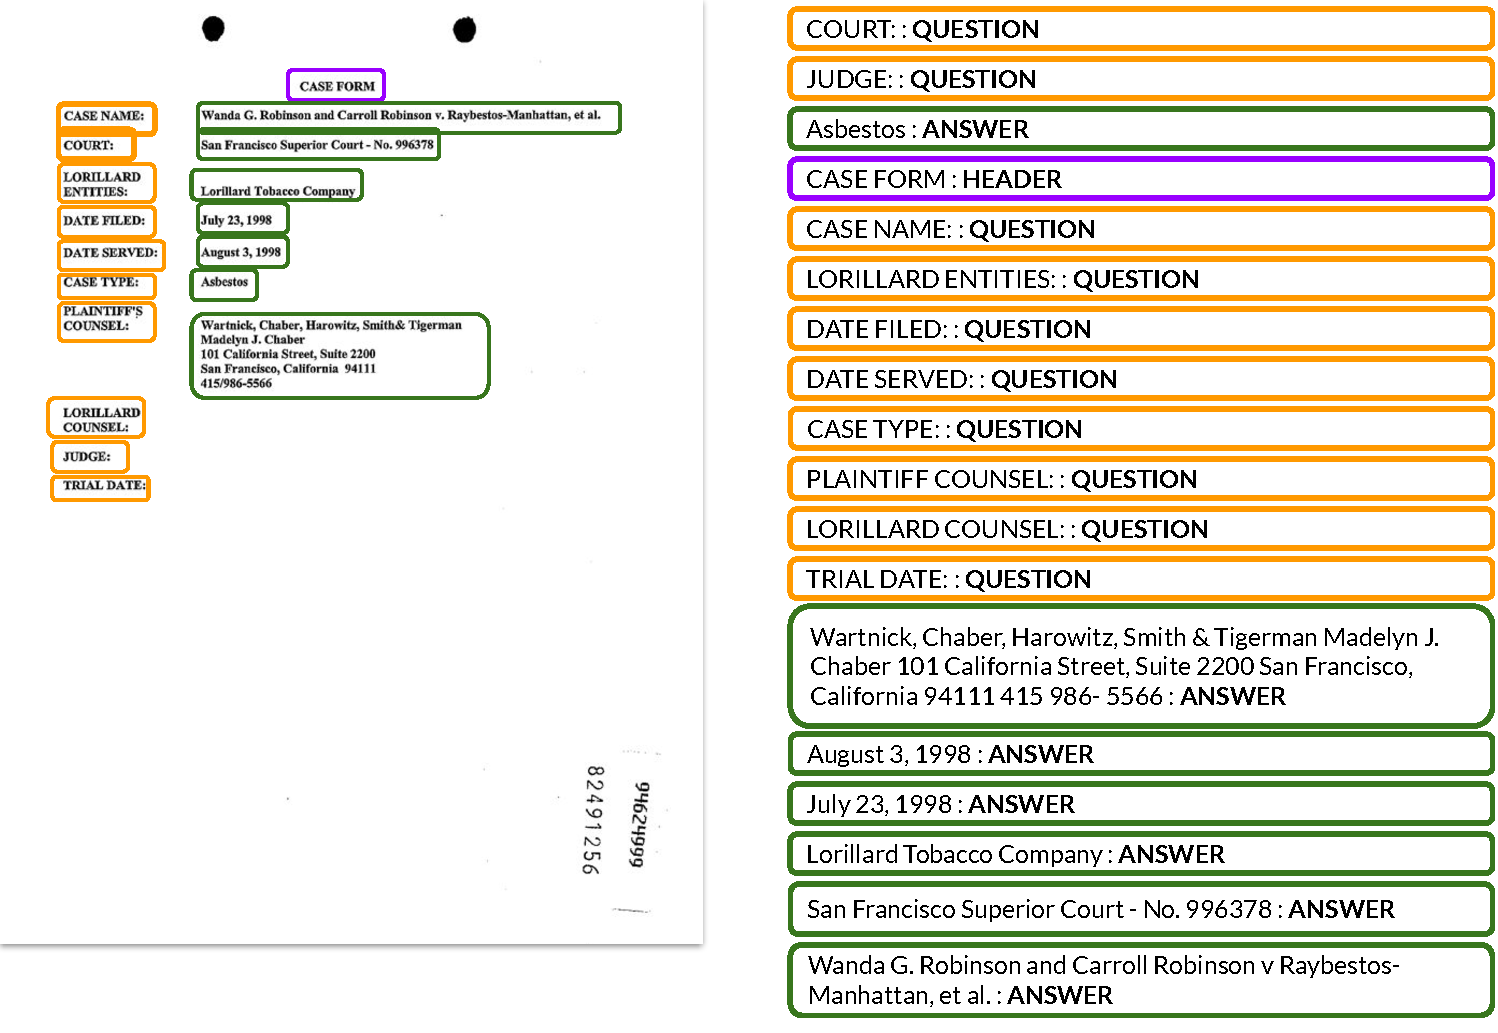
\includegraphics[width=\textwidth]{images/chapter4/funsd_sample_and_output.pdf}
%     \caption{FUNSD}
%   \end{subfigure}
%   \begin{subfigure}[b]{0.4\textwidth}
%     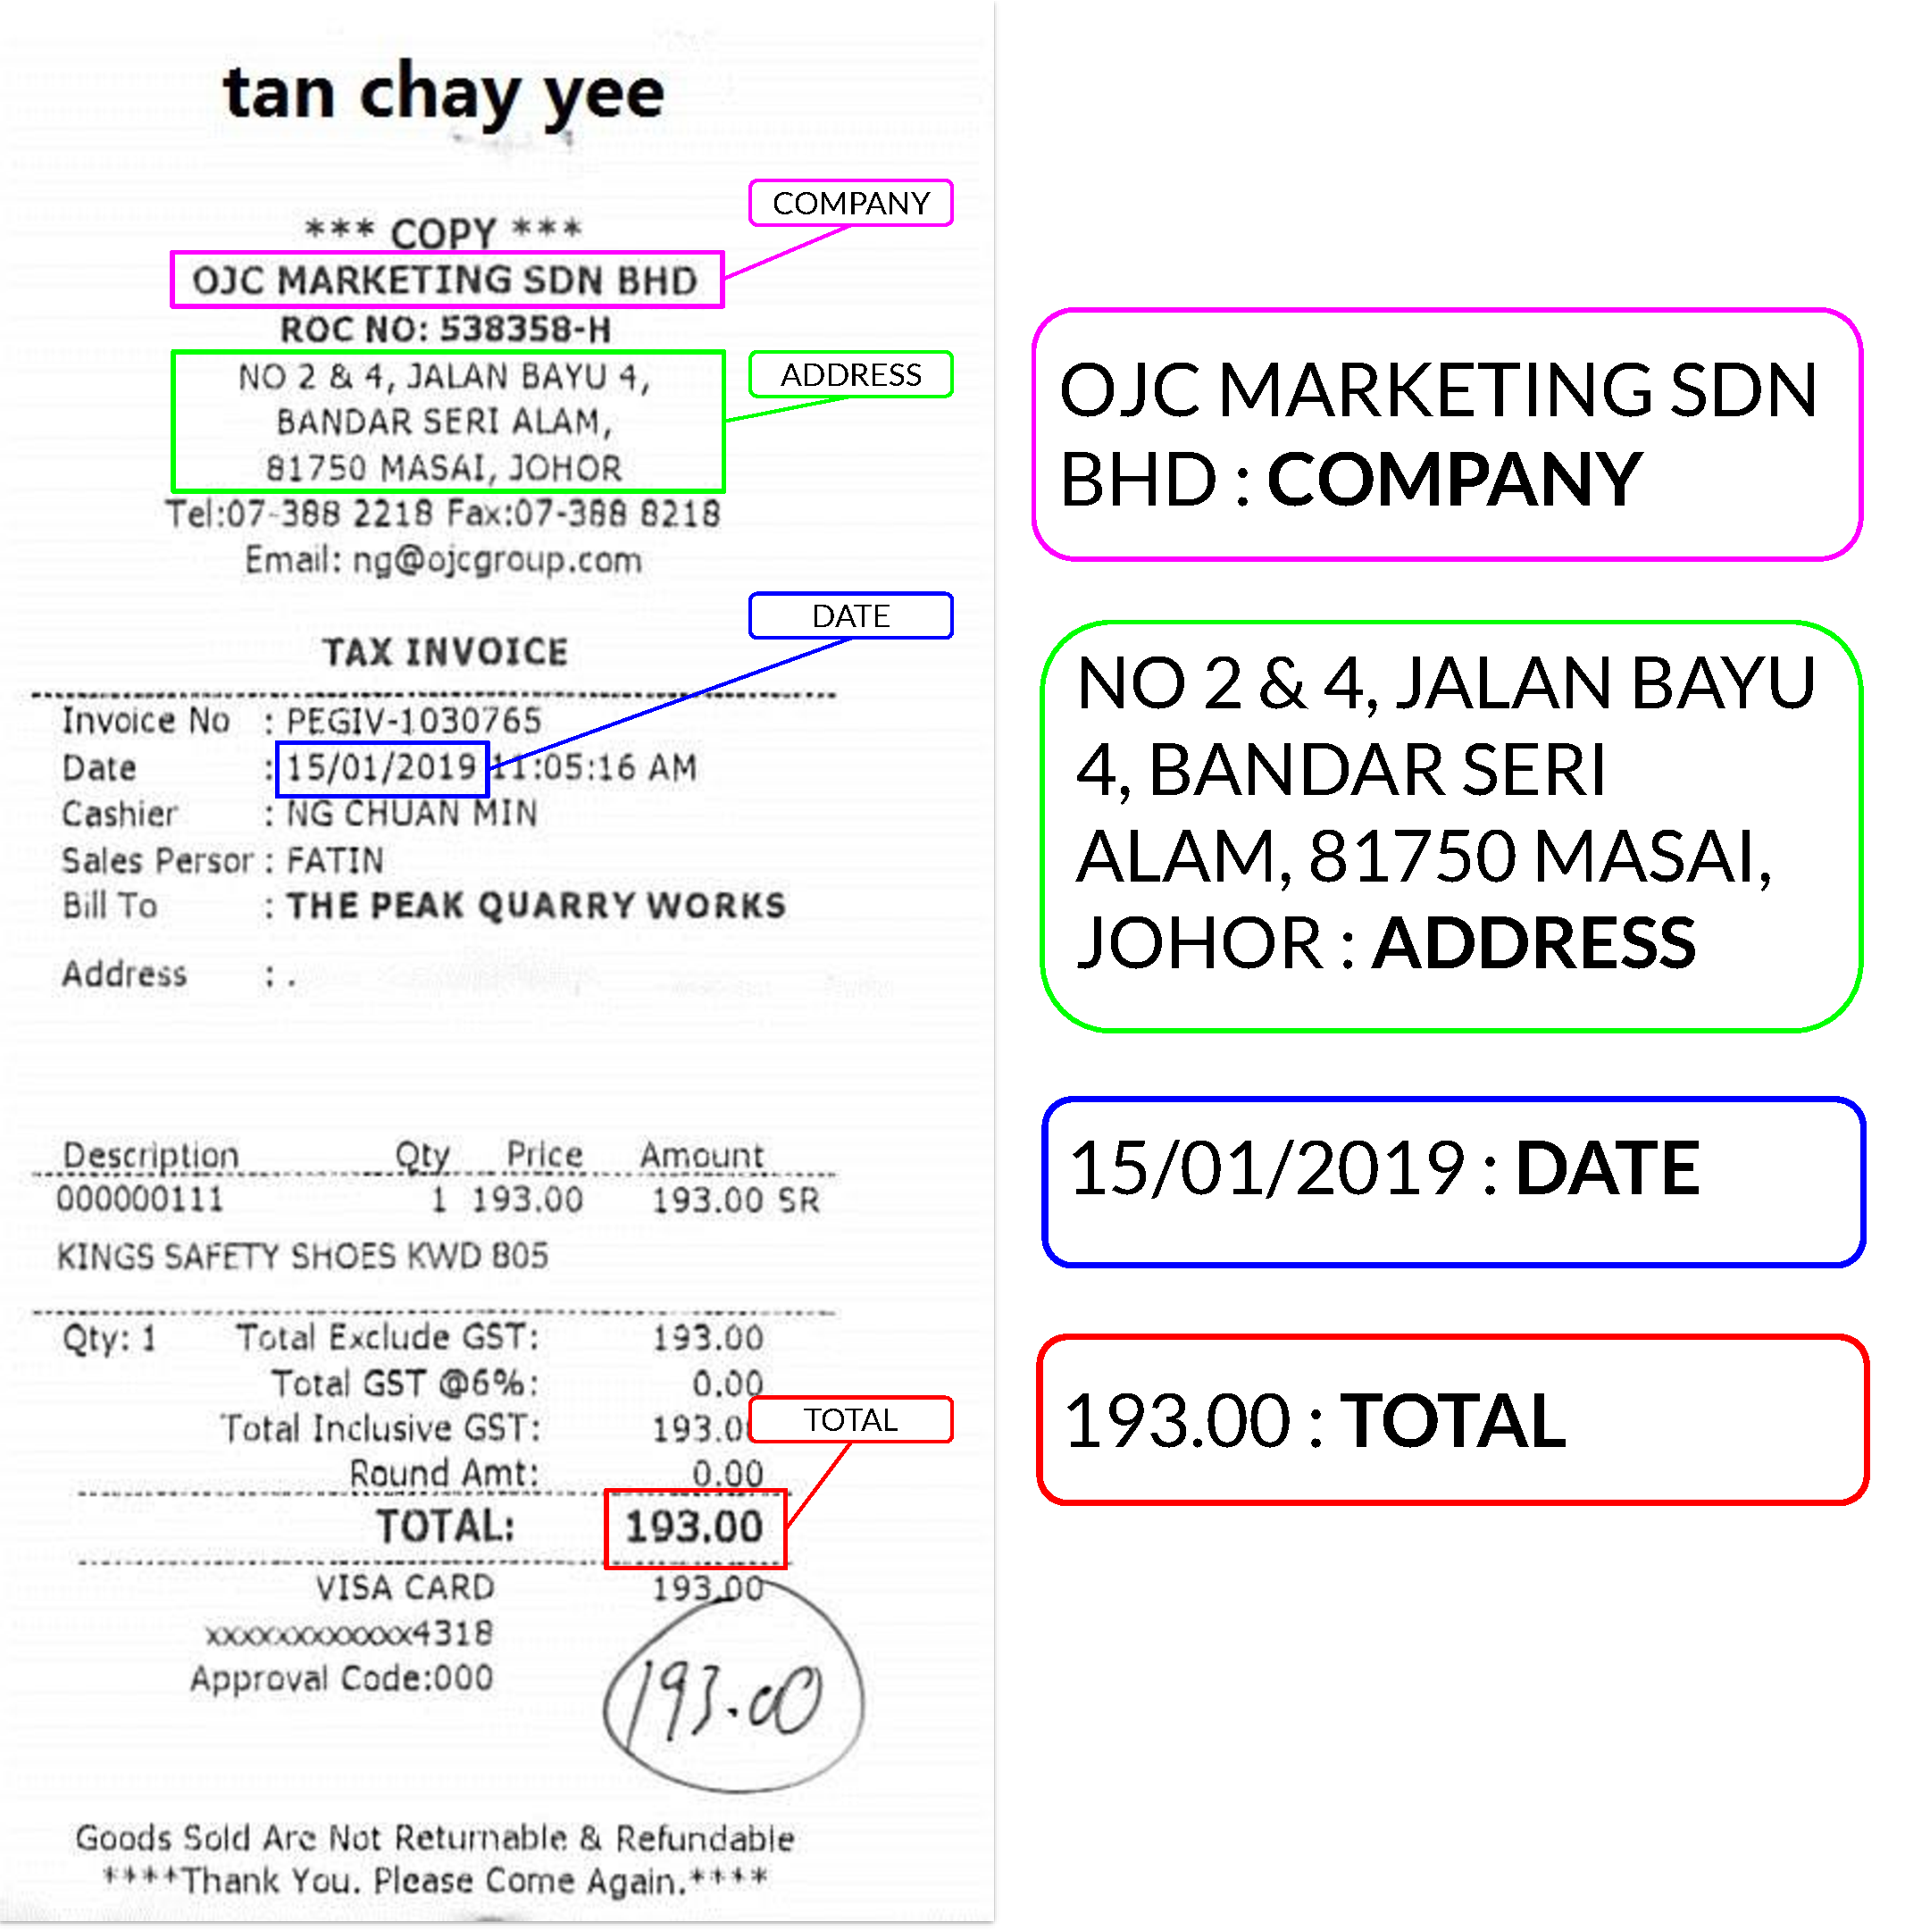
\includegraphics[width=\textwidth]{images/chapter4/sroie_sample_and_output.pdf}
%     \caption{SROIE}
%   \end{subfigure}
%   \begin{subfigure}[b]{0.6\textwidth}
%     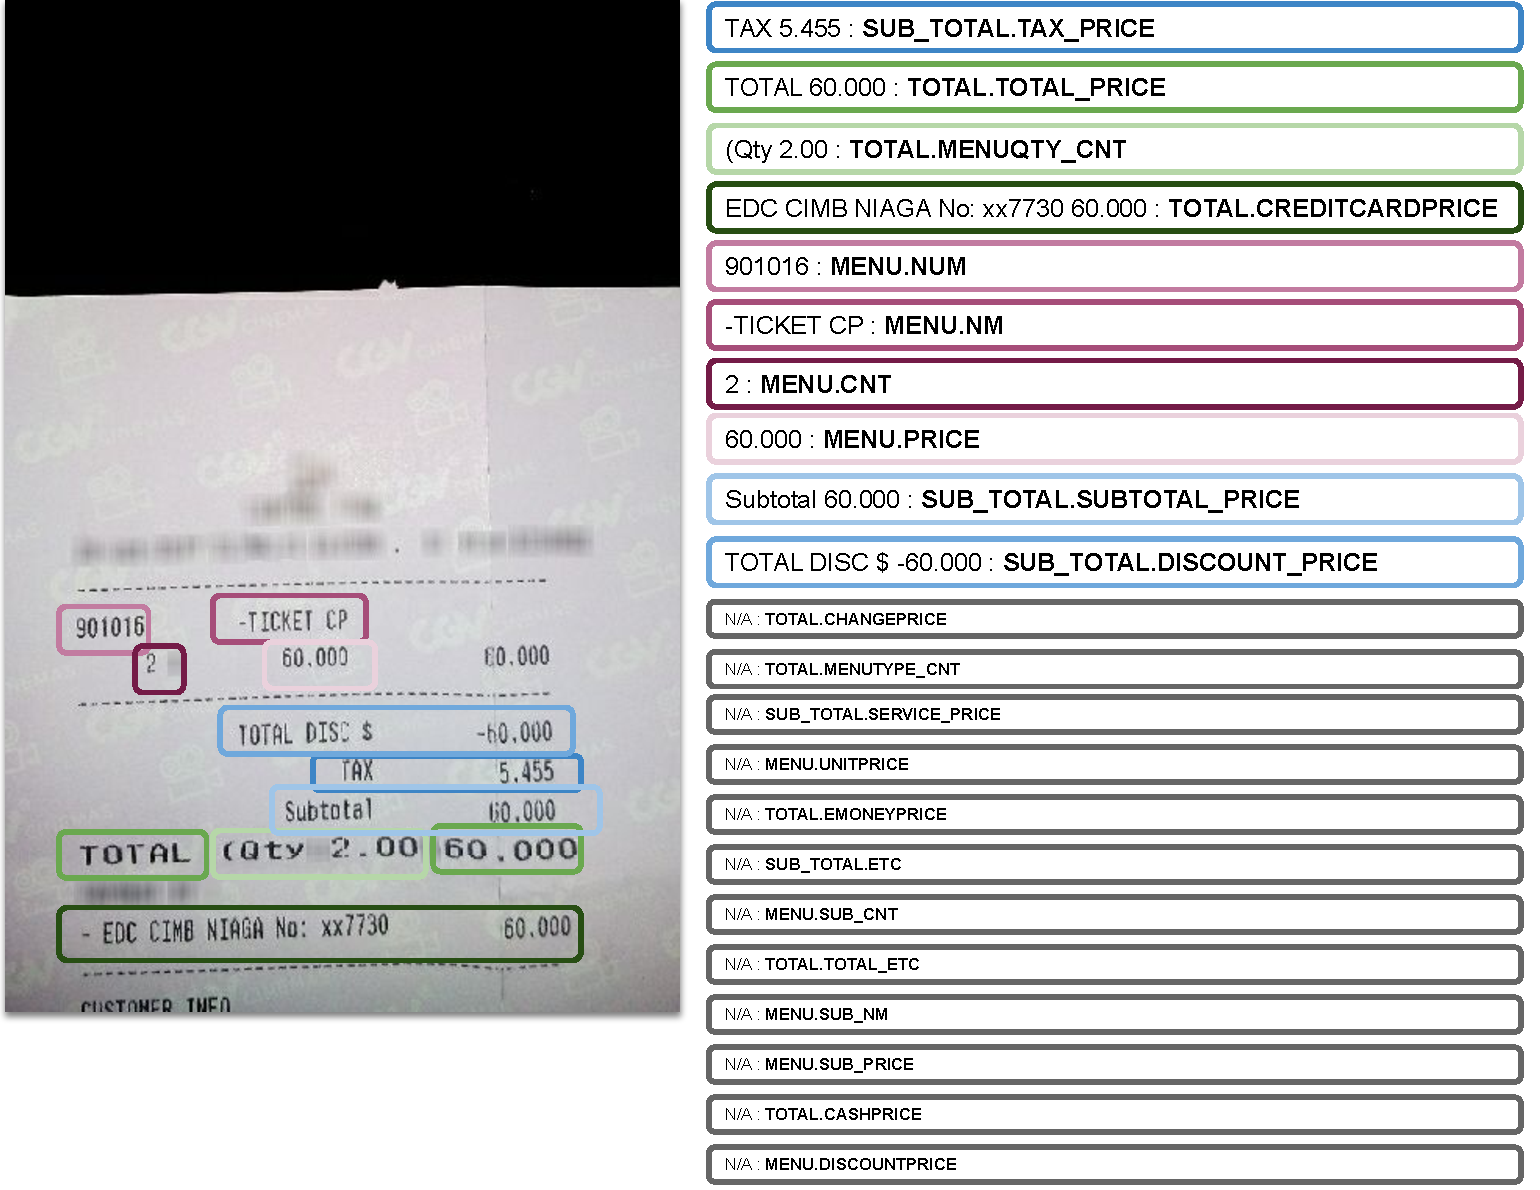
\includegraphics[width=\textwidth]{images/chapter4/cord_sample_and_output.pdf}
%     \caption{CORD}
%   \end{subfigure}
%   \caption{Example document from FUNSD (a), SROIE (b), and CORD (c), accompanied by their corresponding target sequences that include the entities to be extracted paired with their corresponding keys.}
%     \label{fig:source-target-sample}
% \end{figure}

% \begin{figure}
%   \centering
%   \small
%   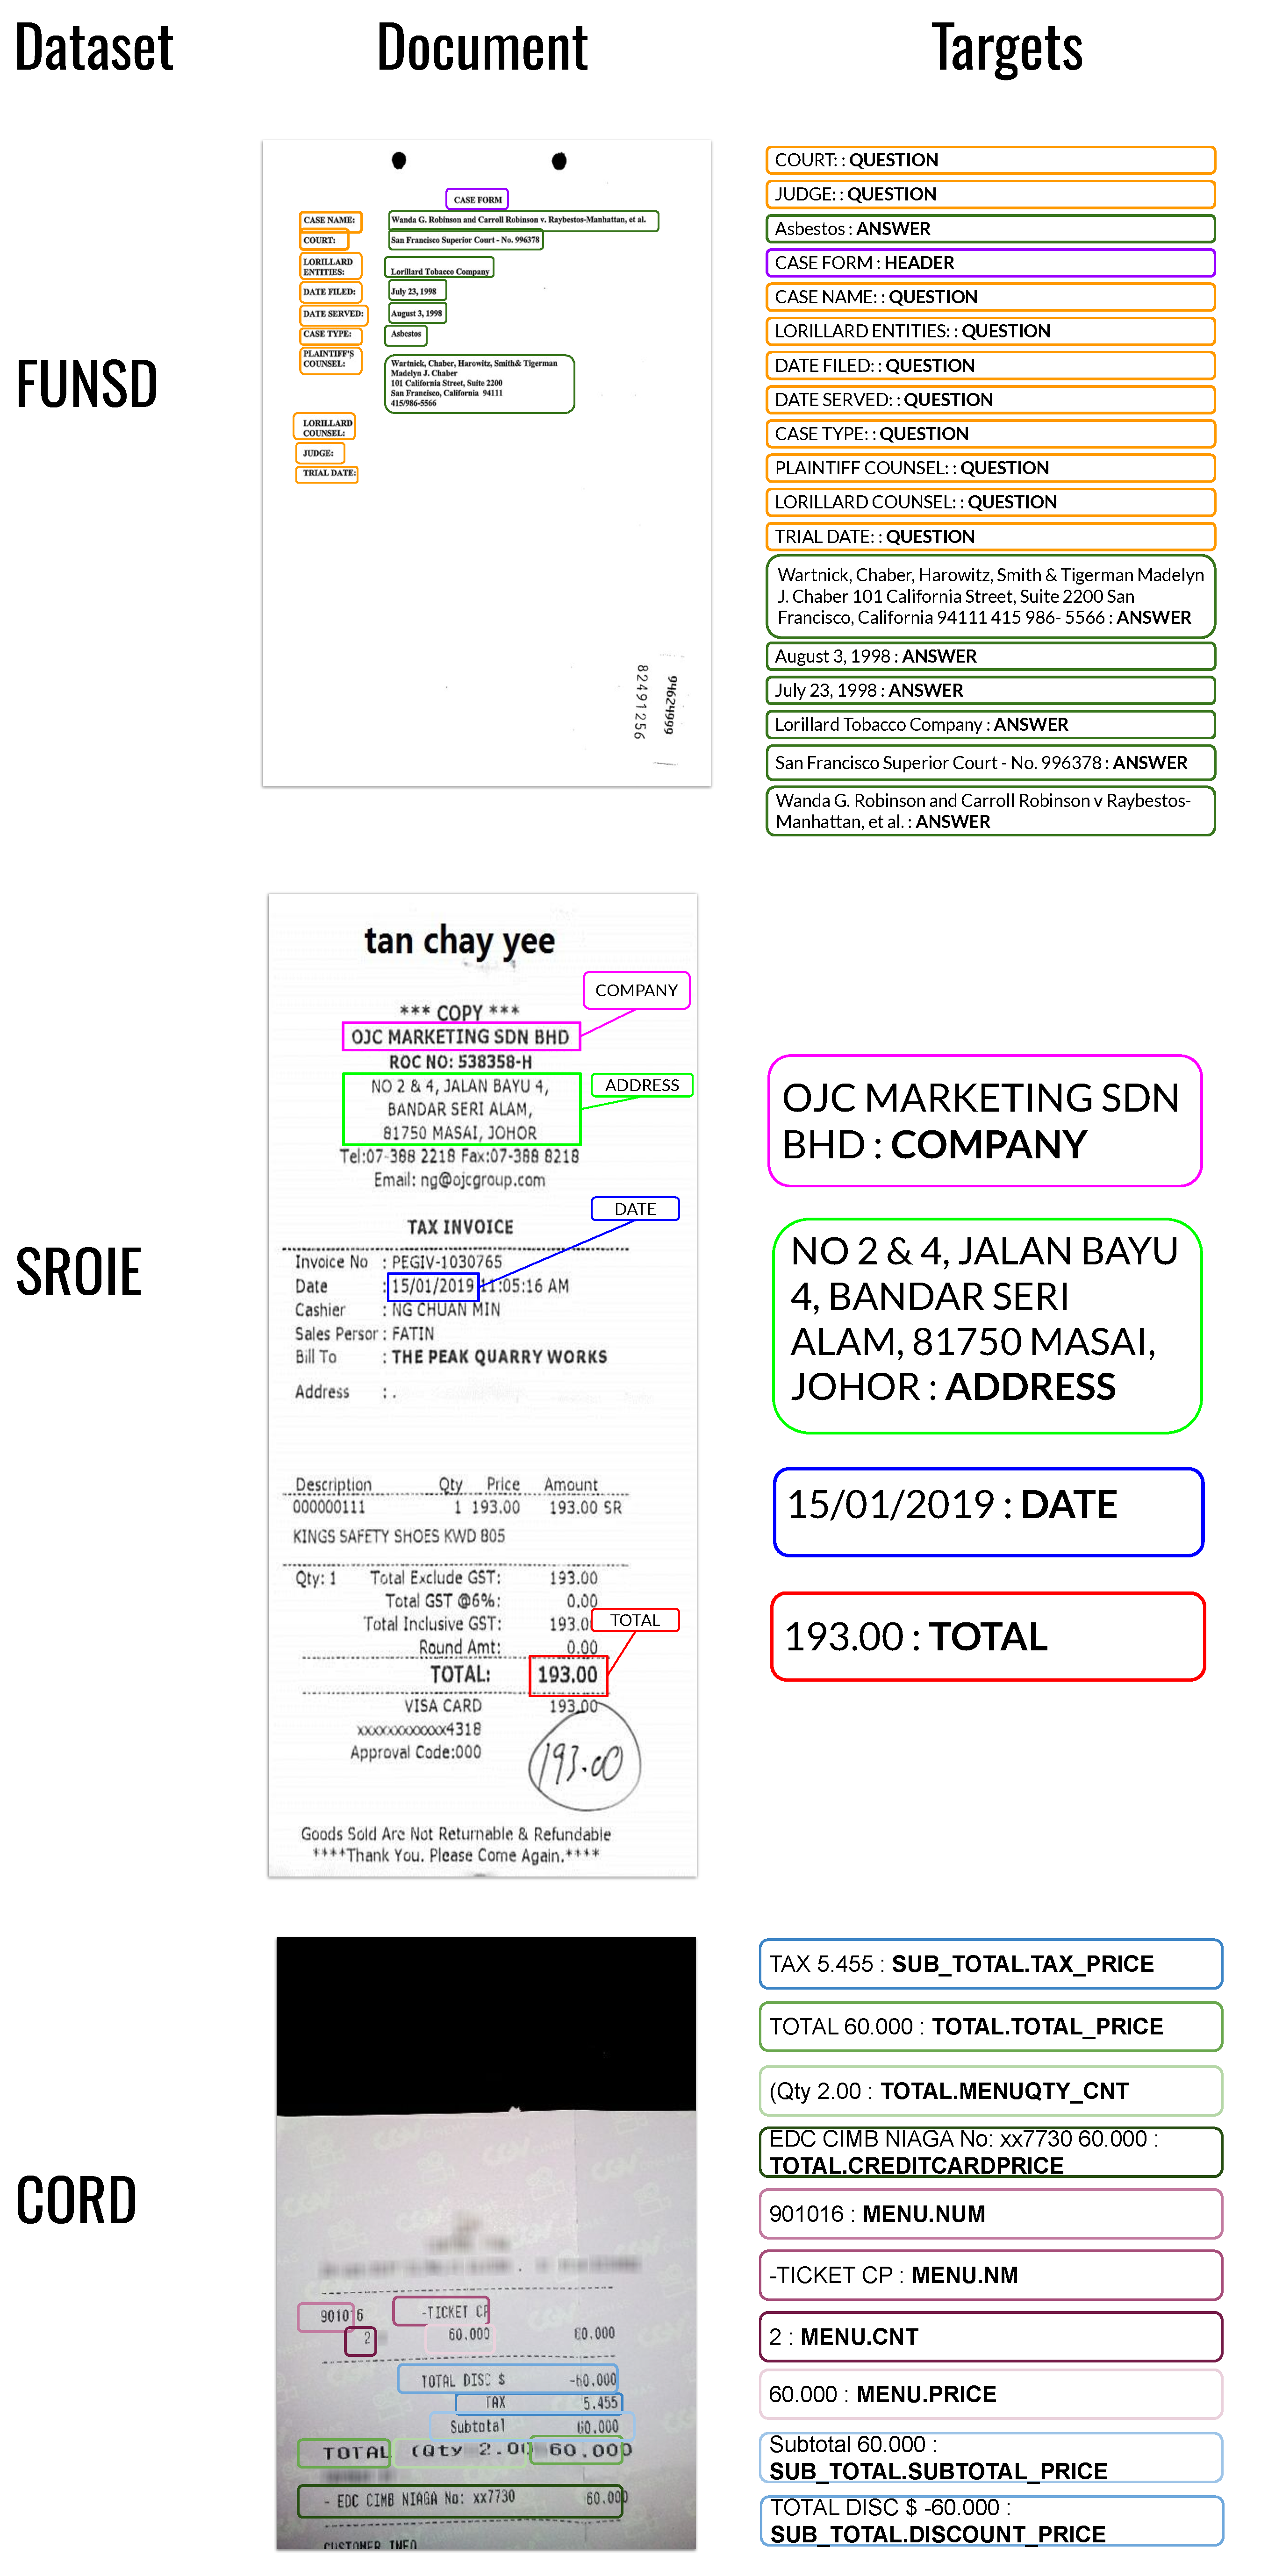
\includegraphics[width=0.6\textwidth]{images/chapter4/all_samples.pdf}
%   \caption{Example document from FUNSD, SROIE, and CORD, accompanied by their corresponding target sequences that include the entities to be extracted paired with their corresponding keys. Best viewed in color.}
%   \label{fig:source-target-sample}
% \end{figure}
\begin{table}[h!]
  \centering
  \begin{tabular}{  c | c | c  }
    Dataset & Document & Targets \\ \hline
    FUNSD
    & 
    \begin{minipage}{.2\textwidth}
      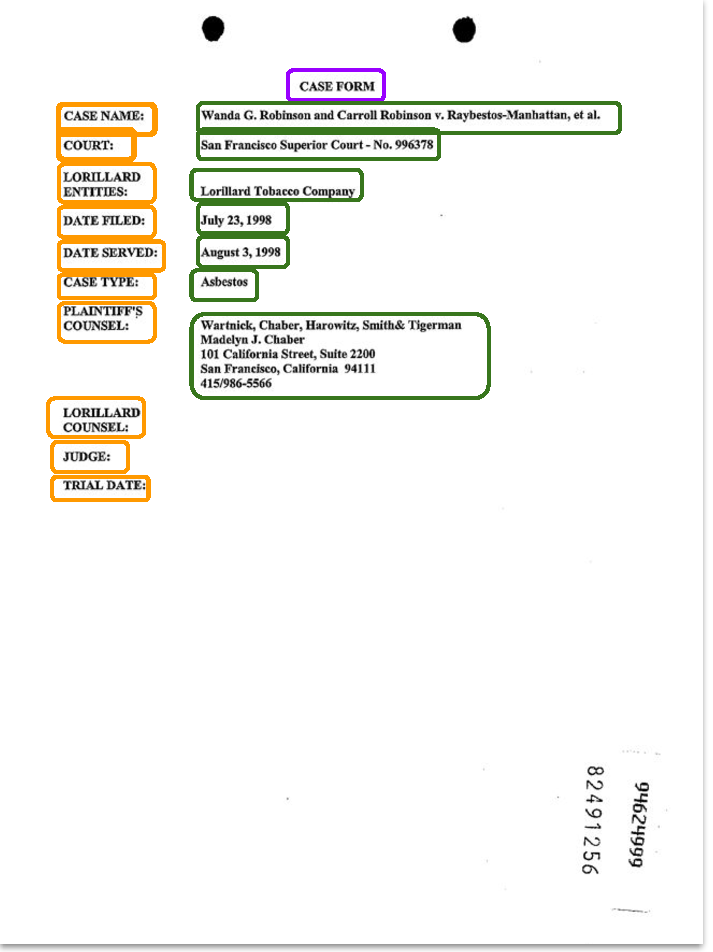
\includegraphics[width=\linewidth]{images/chapter4/funsd_sample.pdf}
    \end{minipage}
    &
    \begin{minipage}{.2\textwidth}
      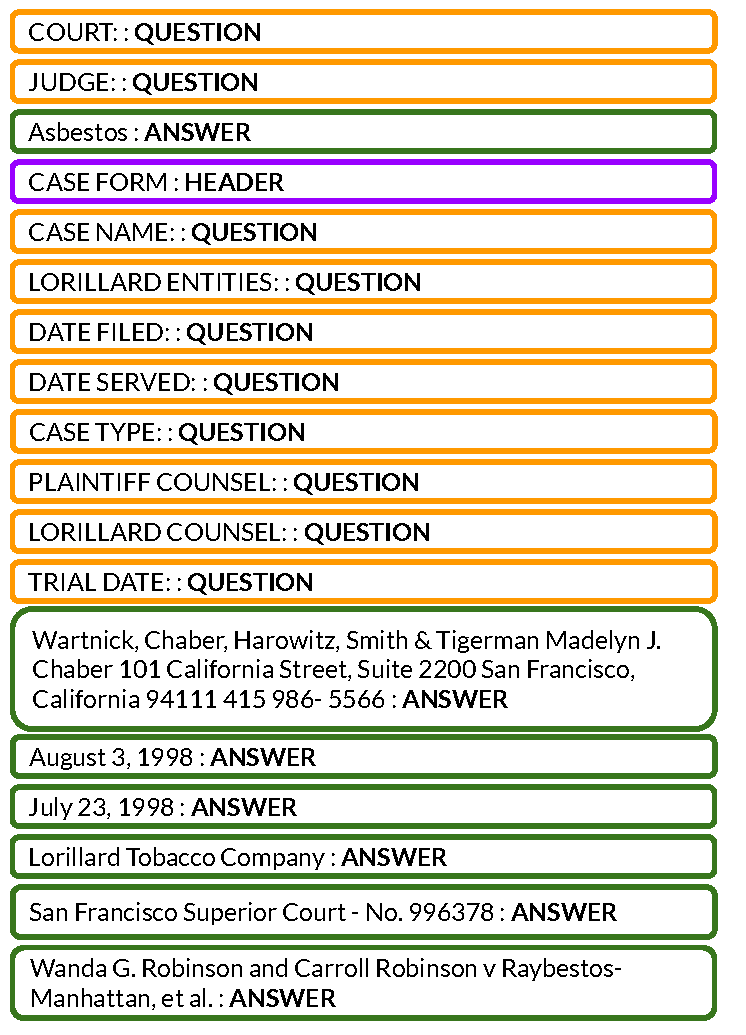
\includegraphics[width=\linewidth]{images/chapter4/funsd_targets.pdf}
    \end{minipage} \\
    \hline 
    SROIE & 
    \begin{minipage}{.2\textwidth}
      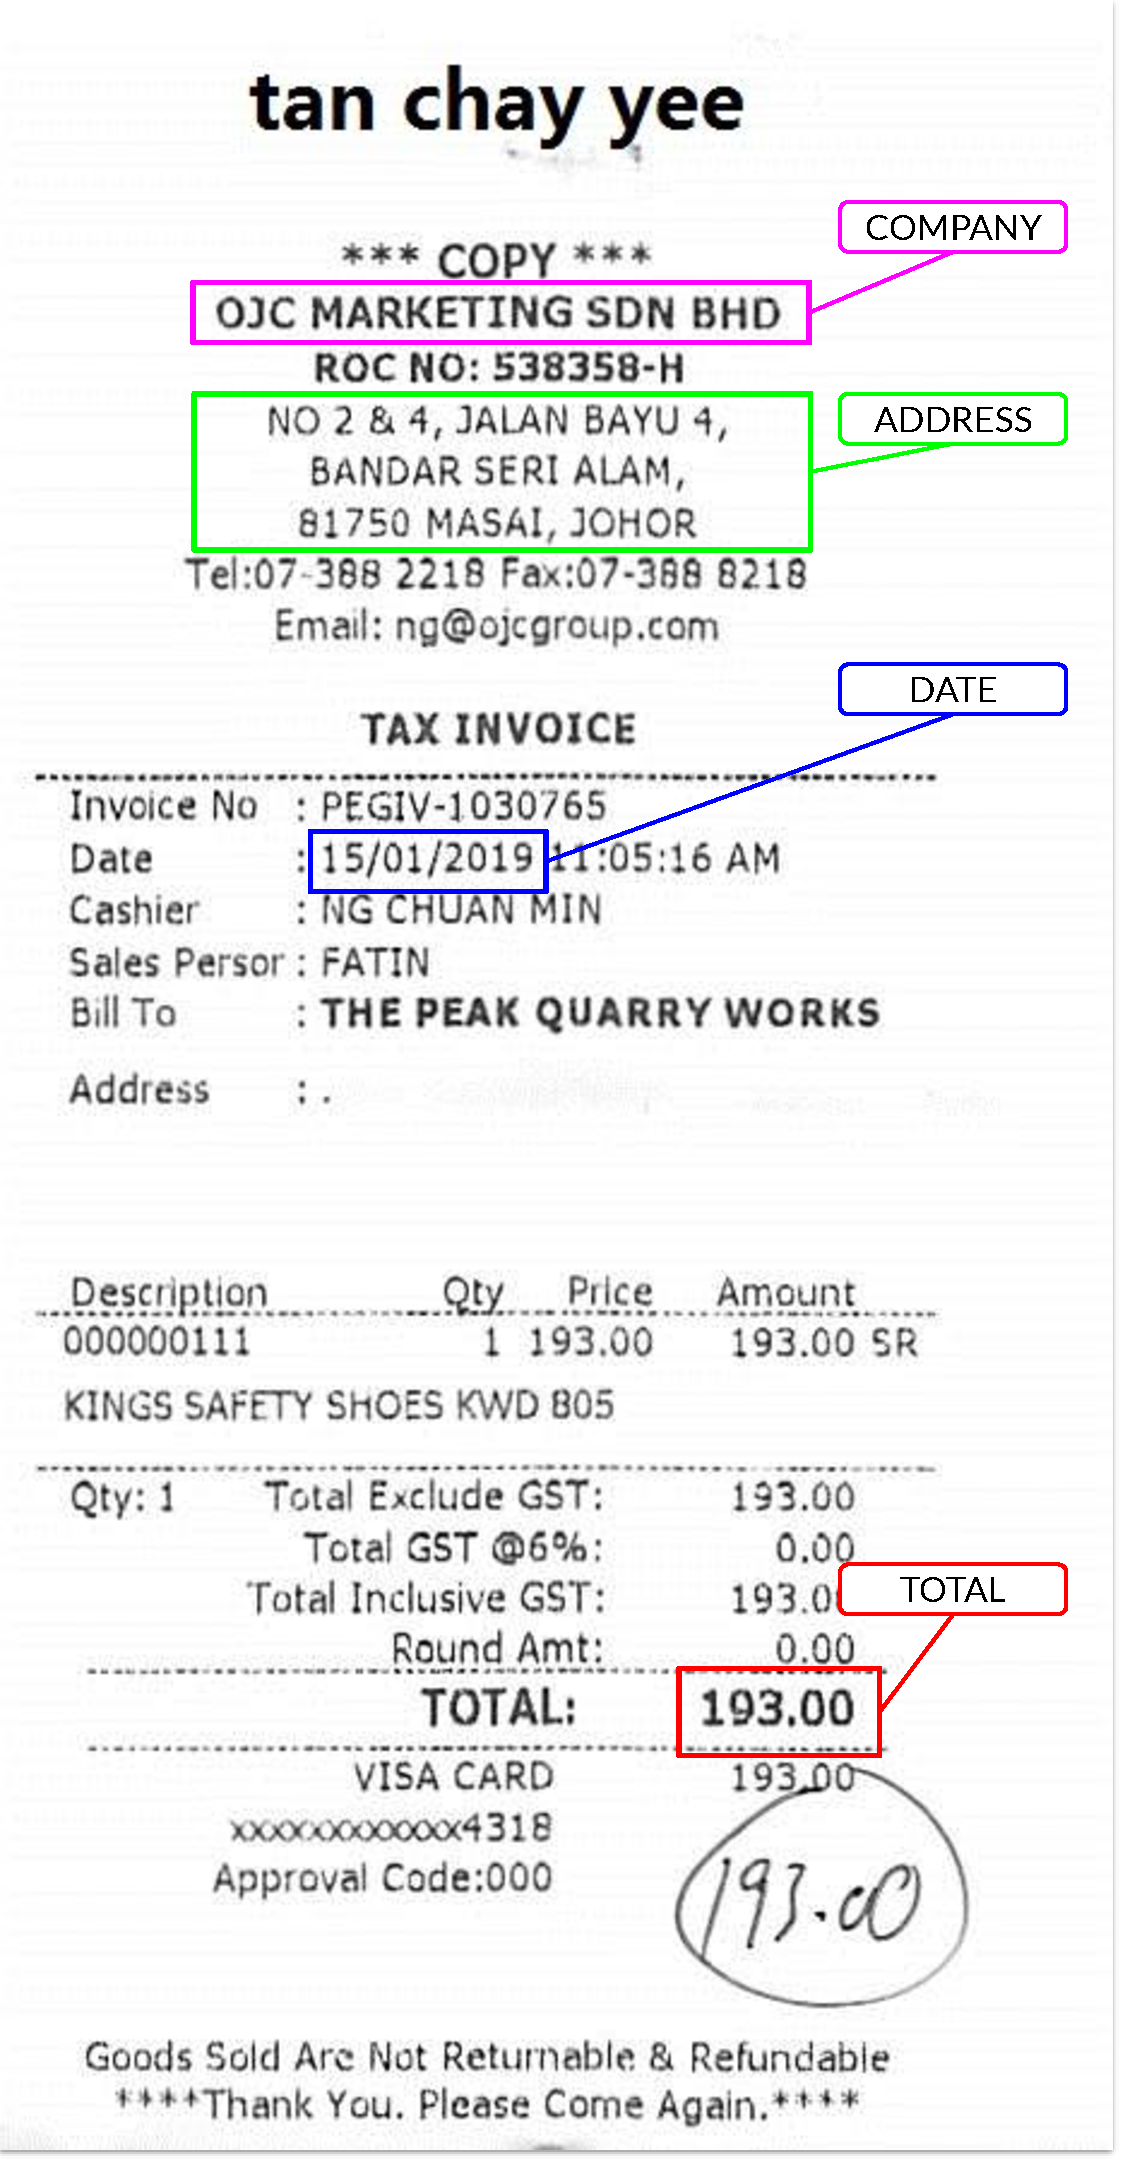
\includegraphics[width=\linewidth]{images/chapter4/sroie_sample.pdf}
    \end{minipage}
    &
    \begin{minipage}{.2\textwidth}
      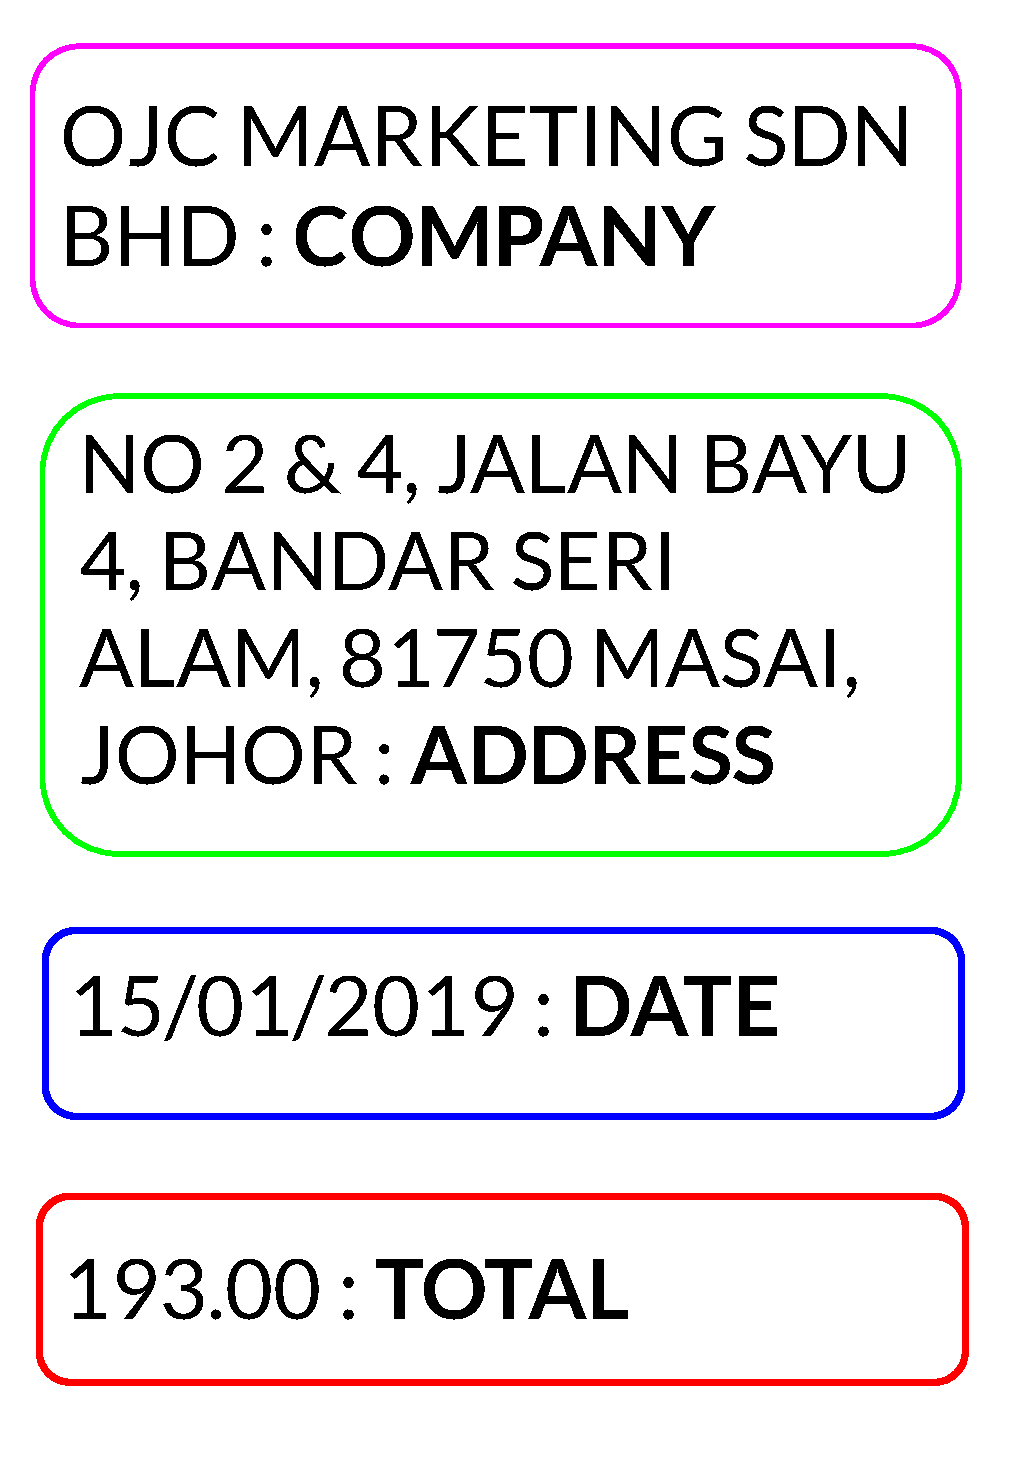
\includegraphics[width=\linewidth]{images/chapter4/sroie_targets.pdf}
    \end{minipage} \\
    \hline 
    CORD & 
    \begin{minipage}{.2\textwidth}
      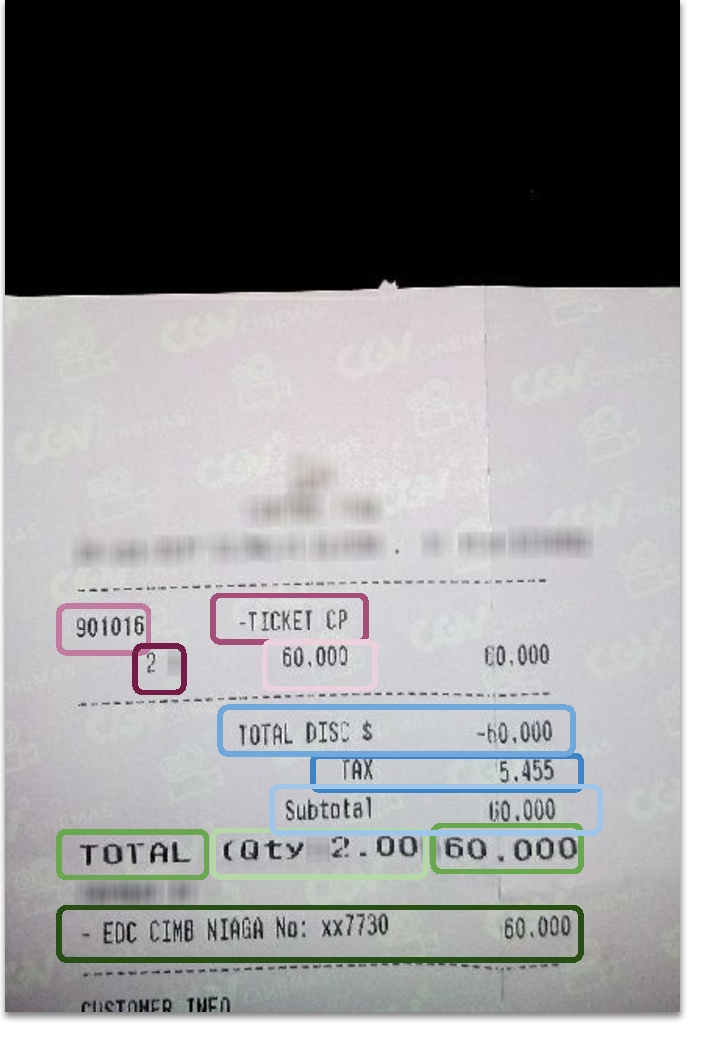
\includegraphics[width=\linewidth]{images/chapter4/cord_sample.pdf}
    \end{minipage}
    &
    \begin{minipage}{.2\textwidth}
      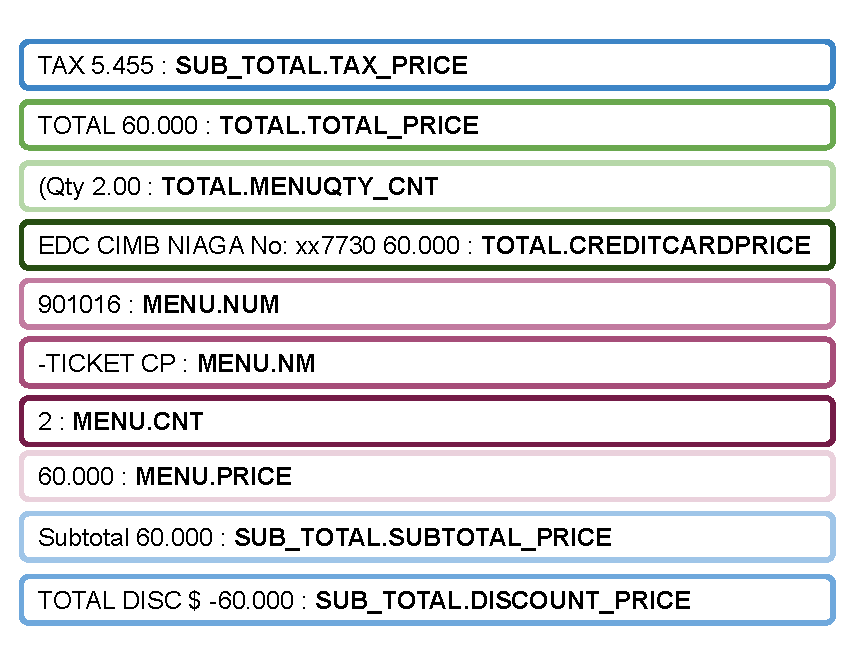
\includegraphics[width=\linewidth]{images/chapter4/cord_targets.pdf}
    \end{minipage}
    \\
  \end{tabular}
  \caption{Example document from FUNSD, SROIE, and CORD, accompanied by their corresponding target sequences that include the entities to be extracted paired with their corresponding keys. Best viewed in color.}
  \label{fig:source-target-sample}
\end{table}

\section{Results and Discussion}

\subsection{Next Token Position Prediction}
\label{section:layout2pos-results-ntpp}

\begin{table}
  \centering
  \small
  \begin{adjustbox}{max width=\textwidth}
  \begin{threeparttable}
  \begin{tabular}{cccc}
      \toprule
          Number of Layers & Pre-training Dataset & Accuracy \\ 
      \midrule
          1                & IIT-CDIP             & 67.10\%  \\
          1                & ReadingBank          & 89.37\%  \\
          2                & ReadingBank          & \textbf{95.86}\%   \\
      \bottomrule
  \end{tabular}
  \end{threeparttable}
  \end{adjustbox}
  \caption{Accuracy in predicting the next token for pairs sourced from ReadingBank, which were not used for pre-training. Selected pairs are considered "difficult", meaning that the tokens are positioned on different lines.}
  \label{table:next-token-prediction-results}
\end{table}

We first evaluate the performance of the Layout2Pos module by computing the accuracy of Next Token Position Prediction. Recalling that the IIT-CDIP dataset is not considered reliable, this evaluation is conducted on a set of pairs of consecutive tokens derived from 100 examples from ReadingBank, which were not used in the pre-training phase. Specifically, we curated pairs categorized as "difficult", where the tokens are positioned on different lines, making a raster-scan approach ineffective. This choice demands the model to leverage layout information to accurately predict the next token in these scenarios.

In these experiments, we exclusively train and evaluate Layout2Pos, omitting the encoder-decoder architecture. For each token, we compute accuracy by comparing the position of its subsequent token with the position of the token associated with the highest logit according to Layout2Pos. We vary the number of layers and the pre-training dataset used. 

Performance is reported in Table~\ref{table:next-token-prediction-results}. Notably, pre-training Layout2Pos on ReadingBank compared to IIT-CDIP yields an increase of over 22\% in accuracy. Additionally, our results indicate that augmenting the number of layers in Layout2Pos results in a notable increase of over 6\% in accuracy. These results highlight the significance of using documents with accurate reading orders and contextualizing layout information to produce position embeddings able to capture the reading order of documents.

\subsection{Visual Information Extraction}

\begin{table*}[h]
  \centering
  \small
  \begin{adjustbox}{max width=\textwidth}
  \begin{threeparttable}
  \begin{tabular}{lllcccccccccc}
      \toprule
       &   & & & &  & &  \multicolumn{4}{c}{\textbf{Rate}} \\ 
       \textbf{Dataset} & \textbf{\shortstack{Reading\\Order}} & \textbf{Model} & & \textbf{Prec.} & \textbf{Rec.} &   \textbf{F1} & \rotatebox{-90}{\textbf{Repetition}} & \rotatebox{-90}{\textbf{Hallucination}} & \rotatebox{-90}{\textbf{Wrong Label}} & \rotatebox{-90}{\textbf{Omission}} & \rotatebox{-90}{\textbf{Non-entity}} \\
      \midrule
      \multirow{6}{*}{FUNSD} & \multirow{4}{*}{Original} & LayoutLM  \citep{xu2020layoutlm} & & 75.91 & 80.54 &	78.16 & \cellcolor[gray]{0.9} & \cellcolor[gray]{0.9} & \cellcolor[gray]{0.9} & \cellcolor[gray]{0.9} &  \cellcolor[gray]{0.9} \\
      & & LayoutLMv2-no-visual             &  & 78.58 &	81.49 &	80.01 & \cellcolor[gray]{0.9} & \cellcolor[gray]{0.9} & \cellcolor[gray]{0.9} & \cellcolor[gray]{0.9} &  \cellcolor[gray]{0.9} \\  
      & & BART+2D & & 83.74 &	86.55 &	\textbf{85.12} &  2.67 & 1.32 &	45.76 &	39.06 &	1.19 \\ 
      & & BART+Layout2Pos & & 80.62 &	80.10 &	80.36 &	2.56 & 5.50 & 22.88 & 57.11 &	3.96  \\
      \cline{2-12}
      % & Shuffled & BART+2D & & 77.82 & 82.16 & 79.93 & 2.89 & 2.15 & 48.37 & 34.68 & 3.25 \\
      & \multirow{2}{*}{Shuffled} & BART+2D & & 77.82 & 82.16 & 79.93 & 2.89 & 2.15 & 48.37 & 34.68 & 3.25 \\
      & & BART+Layout2Pos & & 80.84 &	80.98 &	\textbf{81.13} & 2.37 & 5.31 & 22.30 & 58.05 & 3.97 \\ 
      \midrule
      \multirow{6}{*}{SROIE} & \multirow{4}{*}{Original} & LayoutLM  \citep{xu2020layoutlm} &  & 90.74 & 93.95 & 92.32 & \cellcolor[gray]{0.9} & \cellcolor[gray]{0.9} & \cellcolor[gray]{0.9} & \cellcolor[gray]{0.9} & \cellcolor[gray]{0.9} \\ 
      & & LayoutLMv2-no-visual             &  & 93.20 &	93.88 &	93.54 & \cellcolor[gray]{0.9} & \cellcolor[gray]{0.9} & \cellcolor[gray]{0.9} & \cellcolor[gray]{0.9} &  \cellcolor[gray]{0.9} \\
      & & BART+2D & & 93.46 &	93.73 &	\textbf{93.60} & 0.00 &	0.29 &	0.00 &	18.11 &	2.64  \\
      & & BART+Layout2Pos & & 93.20 &	93.80 &	93.50 & 0.00 &	0.58 &	0.29 &	17.03 &	3.43 \\
      \cline{2-12}
      % & Shuffled & BART+2D & & 80.58 & 66.33 & 73.13	 &  2.66 & 1.46 & 0.41 & 73.34 & 5.72 \\ 
      & \multirow{2}{*}{Shuffled} & BART+2D & & 80.58 & 66.33 & 73.13	 &  2.66 & 1.46 & 0.41 & 73.34 & 5.72 \\ 
      & & BART+Layout2Pos & & 93.13 &	93.80 &	\textbf{93.45} & 0.0 & 0.58 & 0.29 & 17.03 & 3.43 \\ 
      \midrule
      \multirow{6}{*}{CORD} & \multirow{4}{*}{Original} & LayoutLM  \citep{xu2020layoutlm} & & 93.91 & 95.11 & 94.51 & \cellcolor[gray]{0.9} & \cellcolor[gray]{0.9} & \cellcolor[gray]{0.9} & \cellcolor[gray]{0.9} & \cellcolor[gray]{0.9}  \\ 
      & & LayoutLMv2-no-visual             & & 93.14 &	94.89 &	94.00 & \cellcolor[gray]{0.9} & \cellcolor[gray]{0.9} & \cellcolor[gray]{0.9} & \cellcolor[gray]{0.9} &  \cellcolor[gray]{0.9} \\  
      & & BART+2D & & 95.97 &	94.81 &	\textbf{95.39} & 2.33 & 0.00 & 5.28 & 19.06 &	0.33 \\
      & & BART+Layout2Pos & & 94.56 &	92.71 &	93.62 & 0.99 & 4.37 & 5.40 & 22.83 & 0.40 \\
      \cline{2-12}
      % & Shuffled & BART+2D & & 91.46 & 87.54 & 89.46	 & 4.53 & 0.83 & 26.5 & 35.72 & 0.42	 \\ 
      & \multirow{2}{*}{Shuffled} & BART+2D & & 91.46 & 87.54 & 89.46	 & 4.53 & 0.83 & 26.5 & 35.72 & 0.42	 \\ 
      & & BART+Layout2Pos & & 94.45 & 92.61 &	\textbf{93.51} &  1.10 & 4.37 & 5.38 & 22.75 & 0.40  \\ 
      \bottomrule
  \end{tabular}
  \end{threeparttable}
  \end{adjustbox}
  \caption{Model performance (in \%) on FUNSD, SROIE, and CORD, reported for 1) the original reading order and 2) three shuffled orders (averaged). Best F1 scores for each dataset/reading order are reported in bold.}
  \label{table:visual-information-extraction-results}
\end{table*}


Table~\ref{table:visual-information-extraction-results} reports the performance of all four models on FUNSD, SROIE, and CORD. We find that our sequence-to-sequence models achieve performance that is comparable or even superior to sequence-labeling approaches. This suggests that the sequence-to-sequence approach can match the effectiveness of traditional sequence labeling methods, offering an alternative that is not constrained by the document's content and reading order. On SROIE, BART+Layout2Pos performs on par with its counterpart fed with sequential position information, BART+2D. This suggests that Layout2Pos effectively leverages layout information to generate meaningful position embeddings on SROIE, implying that the reading order provided by OCR is no longer necessary. However, on the other two datasets, BART+Layout2Pos demonstrates lower performance than BART+2D, with a slight underperformance on CORD and a more notable disparity on FUNSD. Additionally, we find that the majority of errors arise from either omitted or mislabeled entities. Overall, both models rarely hallucinate, repeat entities, or identify a text as an entity when it should not be considered as such. 

To measure the impact of reading order on models dependent on it, we evaluate BART+2D and BART+Layout2Pos on test documents with shuffled reading orders. For every test dataset, the reading order of each document is shuffled such that words belonging to the same entity remain grouped together. This process is repeated three times, generating three shuffled test sets for every original test dataset. BART+2D and BART+Layout2Pos, fine-tuned using the reading order provided by the dataset, are then evaluated on each of the shuffled test sets. The resulting scores are then averaged and reported in Table~\ref{table:visual-information-extraction-results}. Results show that altering the reading order, even while ensuring that words belonging to the same entities are kept together, leads to a significant performance decline for BART+2D. Specifically, there is a F1-score drop of 5.19 and 5.93 for FUNSD and CORD, respectively, and a notable decrease of 20.84 for SROIE. In contrast, such variations have no effect on BART+Layout2Pos, as the model is not reliant on reading order.\footnote{While we do observe marginal variations for BART+Layout2Pos, we attribute these differences to the fact that documents longer than the maximum sequence length may be split into sequences different from those obtained with the original reading order.} This highlights the significance of developing methods robust to variations in reading order.

\section{Conclusion}

To derive position embeddings solely from layout information and avoid reading order issues, we propose Layout2Pos—a Transformer-based module that learns the sequential relationships between tokens in a document. We conduct experiments on three benchmarks datasets for visual information extraction, demonstrating the effectiveness of our approach in leveraging layout information to produce meaningful position embeddings. Furthermore, we showcase the significant impact of variations in reading order on models that rely on sequential position information, encouraging research on reading order-independent methods for document understanding tasks. In addition, we introduce novel metrics that offer additional insights into the performance of sequence-to-sequence models for visual information extraction.

Acknowledging the limitations of our study, our sequence-to-sequence approach considers any arrangement of key-value pairs as valid. However, language models trained with teacher forcing tend to favor a single correct output, potentially penalizing valid responses with different entity orders. For future work, we will investigate permutation invariant losses to foster robustness to variation in entity orders. Furthermore, our current model evaluations are limited by their focus on relatively simple datasets and documents of shorter length. Additionally, our analyses have been confined to English language texts. Recognizing these limitations, we plan to enhance the generalizability by including more complex datasets, particularly those featuring longer documents \citep{gralinski2020kleister}. 
